\chapter{Úvod} 

Schopnost inteligentního myšlení je jednou z nejdůležitějších vlasností lidí i zvířat. Vždyť bez inteligence by lidé nedokázali převýšit evolučně zdatnější obyvatele Země. Co to vlastně je? Inteligence se dá chápat jako schopnost (jedince nebo skupiny) klasifikovat a reagovat na okolní vjemy, aktivně s nimi interagovat a dokonce ho využít ve svůj prospěch. Filosofové si již od staletí páry kladou otázku, zda mohou mít stroje vlastní vědomí, stupeň inteligence, či preference. Samotné vědní odvětví umělé inteligence, dále \textit{UI}, bylo postupně rozvíjeno během 20. století, kdy se souběžně s vývojem mj. matematické logiky, teorie algoritmů a především vývojem výpočetní techniky vůbec odkrývaly možnosti UI jako stále rostoucí vědní displíny.

Cílem této práce je vytvořit inteligentní entitu, agenta, který by dokázal pokořit tak složitý rozhodovací problém, jakým je hra Ms. Pacman. Svět her je pro umělou inteligenci jedno z velkých témat. Hry byly jako zdroje střetu zájmů oponentů zkoumány již v první pol. 20. století. John von Neumann a Oskar Morgernstern na tyto konfliktní problémy nahlíželi jako na matematické příklady, které se dají analyzovat, sestavit jim matematický model a pomocí výpočtů se snažit nalézt optimální strategie pro každého svého účastníka. Hra by nemohla být zábavná, kdyby nepřítel nebyl dostatečně chytrý. Umělá inteligence silného oponenta ve složité hře představuje disciplínu stále otevřenou novým technikám, metodám a experimentům. Výpočetní náročnost takových her staví velkou překážku k vytvoření \textit{ideální} umělé inteligence, vždyť teprve v roce 2016 dokázala umělá inteligece \textbf{porazit člověka} ve hře \textit{Go} \cite{uigo}! UI \textit{AlphaGo} byla navrhnuta v rámci projektu \textit{DeepMind} společnosti \textit{Google} a povedlo se ji historicky poprvé drtivě porazit profesionálního hráče. Ačkoliv se již v minulosti podařilo překonat člověka i ve hře \textit{Šachy}, stále je to však malý krůček pro tak velký svět zajímavých rozhodovacích problémů jakým je i Ms. Pacman. Ms. Pacman patří k těmto složitým úlohám nejen rozměrností stavů, jež ve hře můžou nastat, ale především náhodností chování svých oponentů, duchů. Nelze tedy přesně stanovit, jak se daný duch bude v danou situaci chovat, lze jen jaksi předpokládat (například za použitím pravděpodobnosti) duchovo chování, tudíž je těžší jednoznačne stanovit, jak má agent postupovat v takto dynamickém prostředí. Co kdyby se agent Ms. Pacman postupně na základě vjemů z prostředí \textbf{učil} své budoucí chování v podobné situaci? 
Jedna z kategorií strojového učení (\textit{machine learning}) posilované učení (\textit{reinforcement learning}) je mocný nástroj na aktivní vypočetní stanovení agentovova rozhodnutí na základě aktuální odměny a trestu získaných v daném stavu. Agent Ms. Pacman se bude snažit co nejlépe reagovat na své aktuální okolí tak, aby jeho inteligence překonala problematiku náhodnosti a vypočetní náročnosti této hry. Kvalita agenta bude srovnána s již známými metodami řešení podobných problémů. Dále se práce zaměří na podobné problémy jako je Ms. Pacman a na nich otestuje kvalitu inteligence agenta.

Práce je tedy rozdělena na dva velké celky: teoretickou a praktickou část. Teoretická část práce seznamuje čtenáře se základními pojmy a metodami hraní her v kapitole \ref{teorie:metodyapojmy} a to tak, aby na ně následně mohla navázat nejdůležitější teoretická kapitola \ref{teorie:uciciagent} zaměřující se na důležitou vlastnost agenta -- schopnost učení. Tato kapitola nejdříve pojednává o racionalitě hráče v sekci \ref{sec:racionalita} a popisuje pojem \textit{Markovský rozhodovacích proces} v sekci \ref{sec:mdp}. S těmito pojmy pak pracují již sekce jednotlivých algoritmů UI, například finální vylepšení Q-Learningu: \textit{Aproximační Q-Learning} \ref{sec:qlearning}. Předěl mezi teoretickou a praktickou částí je kapitola \ref{anavrh}, která prakticky rozebírá hru Ms. Pacman a již se detailně věnuje návrhům všech metod zvolených pro implementaci a otestování na demu Ms. Pacman. Praktická část pokračuje implementační kapitolou \ref{realizace}, která popisuje objekový návrh aplikace a především prezentuje implementovaná řešení jednotlivých metod. Kapitola se zaměřuje i na zmíněné další \textit{gridworld} problémy zkoumatelné z hlediska UI, pro které lze také názorně použít zvolené algoritmy. Implementační kapitolu uzavírá popis implementace agenta pro metodu \textit{Aproximační Q-Learning}. Poslední částí práce je kapitola experimentální charakteru \ref{exper}, která se zaměřuje na porovnání jednotlivých agentů na různých typech problémů (vč. Ms. Pacman) a obsahuje finální srovnání časové a vypočetní náročnosti algoritmů.

\chapter{Metody hraní her}
\label{teorie:metodyapojmy}
Tato kapitola si klade za cíl seznámit čtenáře s metodami hraní her. Hry úzce souvisí s metodami řešení úloh, zahrnují tedy snahu dostat se z počátečního stavu do cílového, např. za použití posloupnosti nějakých pravidel. 

\section{Základní pojmy}

\subsection*{Stavový prostor}
Stavový prostor \cite{AI1} je množina všech stavů, které mohou ve hře nastat. Stavový prostor lze reprezentovat jako orientovaný graf, jehož \textit{uzly} představují jednotlivé pozice ve hře (stavy) a orientované hrany přechody mezi jednotlivými stavy, tedy přípustné tahy ve hře. První uzel se nazývá \textit{kořen}, koncové uzly, \textit{listy}, pak reprezentují koncové pozice ve hře (cíle, stavy). Na obrázku \ref{img:stavp} lze vidět ukázku omezeného (zjednodušeného) stavového prostoru hry Pacman. Velikost takto velmi omezeného stavového prostoru musí vzít v potaz: rozměry 2D hracího pole, 4 možné směry pohybu Pacmana a fakt, zda 8 kuliček jídla už (ne)bylo snězeno, tedy:  $3 \times 3 \times 2^{8} \times 4 = 9\:216$ (!) stavů a to nebyl brán v potaz ani jediný nepřítel, natožpak reálná velikost hracího pole desky.
\newline
K dosažení každého uzlu je potřeba vydat nějaké úsilí, \textbf{cenu} \cite{AI1}, která tedy udává nezáporné ohodonocení hrany z jednoho uzlu k druhému. \textbf{Hloubka uzlu} \cite{AI1} udává počet hran na cestě od počátečního uzlu k danému uzlu. Kořen má hloubku 0, jeho následníci mají hloubku 1 atp.


\begin{figure}[h]
\begin{center}
  \scalebox{0.7}{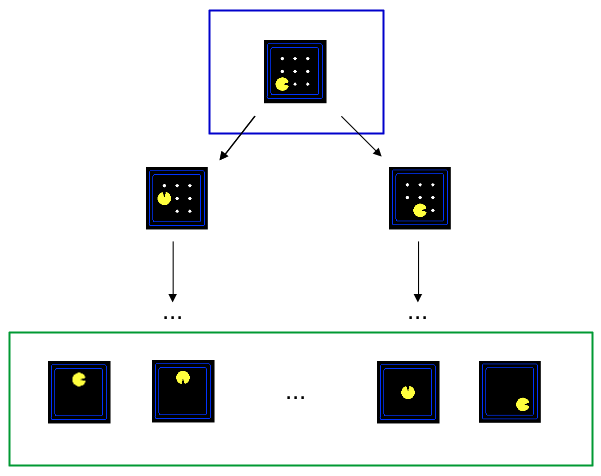
\includegraphics{img/statespace.png}}
  \caption{Ukázka stavového prostoru pro hru Pacman. Každý pohyb Pacmana znamená nový stav hry, tedy uzel. Modrý obdélník ohraničuje počáteční stav, kořen, a zelený obdelník ohraničuje možné koncové stavy, listy.}
  \label{img:stavp}
\end{center}
\end{figure}

\subsection*{Optimální versus nejlepší řešení}
Další důležitou součástí metod řešení úloh je \textbf{hodnotící funkce} (\textit{successor function}) \cite{AI1}. Jedná se o funkci vyhodnocující celkovou cenu od jednoho uzlu k druhému, např. součet ceny a \textit{heuristické funkce}. \textbf{Heuristická funkce} \cite{berkeley} je založena na empirických znalostech (až odhadech) o hře, používaná při prohledávání stavového prostoru. Může to být například vzdálenost Ms. Pacman vůči svému cíli. Podle jejího využití dělíme algoritmy na \textbf{informované} a \textbf{neinformované} \cite{AI1}.
Proč se ale používá heuristika místo jistějšího systematického prohledávání stavového prostoru, které by mělo definovat vlastně \textit{nejlepší} řešení? Je to především kvůli velké vypočetní náročnosti toho způsobu prohledávání a vyhodnocování celého stavového prostoru, který u složitějších problémů nabývá příliš velkých rozměrů, aby se vše stihlo provést, např. v reálném čase při hraní hry. Pokud je heuristika \textit{optimální}, zaručuje zvýšení efektivity a rychlosti.
\newpage
\subsection*{Vlastnosti algoritmů}
Rozlišujeme několik následujících vlastností algoritmů\cite{AI1}:
\begin{itemize}
\item \textbf{Úplnost} – Pokud existuje řešení, je garantováno, že ho algoritmus vrátí?
\item \textbf{Optimálnost} – Je garantováno nalezení nejlepší řešení, tedy řešení s nejmenší cenou?
\item \textbf{Časová složitost} – Kolik uzlů je nutno expandovat? Kolik to zabere času v nejhorším/nejlepším případě/průměrně?
\item \textbf{Prostorová složitost} – Kolik dat je nutno si uchovávat v paměti v nejhorším/nejlepším případě/průměrně?
\end{itemize}

\section{Hry}
\textbf{Hra} (také se označuje jako \textit{adversarial search}) je z matematického hlediska rozhodovací problém, ve kterém figurují 2 a více účastníků, hráčů \cite{AI1}. Hráči se snaží chovat racionálně, viz sekce \ref{sec:racionalita}.
\newline
\textbf{Složité hry} \cite{AI1} jsou hry s tak velkým úplným stavovým prostorem, že by jeho neinformované prohledávání nebylo možné výpočetně zvládnout. Například Šachy, Go, Ms. Pacman. V takových případech je potřeba omezit strom stavového prostoru pomocí hloubky, tedy maximálního počtu kroků dopředu oproti aktuálnímu stavu, a použít \textit{statickou hodnotící funkci}, která určuje \textit{pravděpodobnost} dosažení cíle z aktuálního stavu. Následující metody hraní her potřebují mít úplnou informaci o stavovém prostoru hry.
\subsection*{Minimax}
Metoda \cite{AI1} prohledávání do hloubky s omezením hloubky prohledávání. Hodnotící funkce nám udává určitou \textit{hodnotu} listů $V(s)$, tedy nejlepší výsledek/užitek, kterého lze dosáhnout z aktuálního stavu.
Následně se úrovni hráče při procházení stavového prostoru vybírá \textbf{maximum hodnoty:} $V(s) = \max \: V(s^\prime)$, kde $s^\prime \in naslednici(s)$. 
\newline
Na úrovni protihráče \textbf{minimum hodnoty:} $V(s^\prime) = \min \: V(s)$, kde $s \in naslednici(s^\prime)$. Hráči se takto rekurzivně střídají od listů až po finální výpočtení hodnoty kořene.

\subsection*{AlfaBeta řezy}
Metoda pro zmenšení stavového prostoru \cite{AI1}, odříznutím nadbytečných větví. Využívá dvou \textit{mezí}:
\begin{itemize}
\item \boldmath$\alpha$ reprezentující dolní mez ohodnocení uzlu, tedy tah hráče (zpočátku $\alpha = -\infty $),
\item \boldmath$\beta$ reprezentující horní mez ohodnocení uzlu, tedy tah protihráče (zpočátku $\beta = \infty $).
\end{itemize}
Algoritmus si pamatuje hodnoty svých mezí, a postupně je aktualizuje porovnáváním meze s následníky uzlu aktuální úrovně a to podle toho, na které úrovni se nachází: ($max$ -- aktualizuji $\alpha$ na největší hodnotu následníků, $min$ -- aktualizuji $\beta$ na nejmenší hodnotu následníků). Porovnávání probíhá dokud $\alpha < \beta$, takto se vynechají nadbytečné větve, jejichž procházení již nezmění výslednou cestu. Konečná hodnota kořene je stejná jako u Minimaxu, a pokud by se uzly správně seřadily, výrazně se tím změní vypočetní náročnost algoritmu.
 
\subsection*{Expectimax}
Expectimax \cite{mas} je jednou z možností jak řešit \textbf{hry s neurčitostí} jako je i Ms. Pacman. Hry s neurčitostí také zahrnují střídání hráčů a mají také úplnou informaci o stavu hry, avšak navíc využívají při získání těchto informací \textit{pravděpodobnosti}, které popisují náhodný charakter stavů ve hře. Příkladem jsou hry, kde figuruje házení kostkou nebo např. řízení libovolného robota v reálném světě, kdy se může náhodně pokazit nějaká jeho součástka. Expectimax obohacuje každý tah hráče (jako Minimax) o náhodnost. \textbf{Hodnoty stavů} nyní navíc reflektují průměrnou pravděpodobnost stavů:
\begin{align}
V_{\min}(s) = \sum_{i=0} p_i * \min \: V(s^\prime)
\end{align}
\begin{align}
V_{\max}(s^\prime) = \sum_{i=0} p_i * \max \: V(s^\prime)
\end{align}
kde $s^\prime \in naslednici(s)$ a $p_i$ je pravděpodobnost daného stavu $i$-té úrovně.
\newline
Tyto rovnice udávají tzv. \textbf{očekávaný užitek} (\textit{expected utility}) dané úrovně \cite{mas}. Na obrázku \ref{img:expectimax} lze vidět použití algoritmu.
\newpage

\begin{figure}[!htbp]
\begin{center}
  \scalebox{0.35}{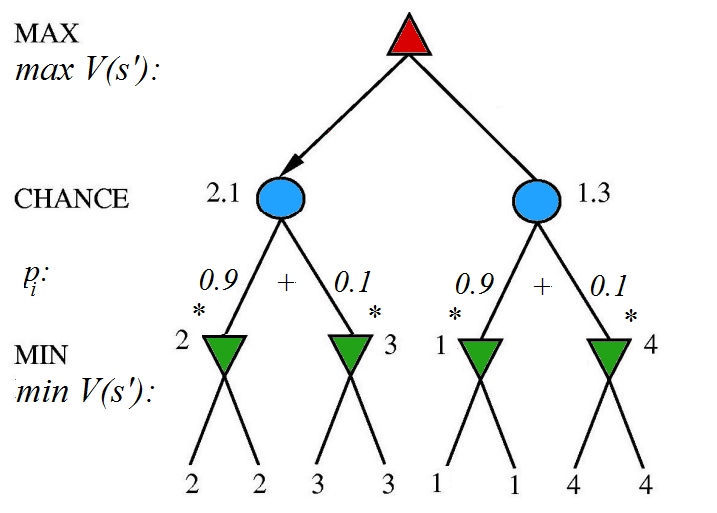
\includegraphics{img/expectimax.png}}
  \caption{Na obrázku lze vidět ukázku vyhodnocování uzlů a výslednou cestu $A_1$, kterou si algoritmus posléze zvolí.}
  \label{img:expectimax}
\end{center}
\end{figure}

\chapter{Učící agent}
\label{teorie:uciciagent}
Tato kapitola se zaměřuje na teoretický podklad hlavního cíle práce, inteligentní formu reaktivního agenta \cite{AI3}.
\section{Reaktivní agent}
Reaktivní agent \cite{AI3} se dá představit jako autonomní bot, který reaguje na své aktuální okolní prostředí. Nebere tedy v potaz následky svého konání. Matematicky lze zapsat \textit{šesticí} \cite{AI3} jako: $(S, T, A, vjem, ukon, akce)$, kde:
\begin{itemize}
\item $S$ je množina okolních stavů agenta,
\item $T, T\subseteq S$ je okolí, které může agent vnímat,
\item $vjem: S \to T$ je agentem právě vnímaný stav okolí ($s \in S$),
\item $A$ je množina možných úkonů, jež může agent v daný stav vykonat,
\item $ukon: A \times A \to S$ je vykonaný úkon, jež má za následek změnu prostředí $S$,
\item $akce: T \to A$ je vybraná akce na základě $vjemu$.
\end{itemize}
Agent představuje účastníka hry (hráče).

\section{Racionalita}
\label{sec:racionalita}
Každý hráč má nějaký cíl a k němu vedoucí strategii. Strategie se skládá z hráčových akcí a voleb, které pro hráče vedou k vlastnímu užitku (\textit{utility}), potažmo výhře. Hráč se potýká s různými stavy ve hře a snaží se z nich vytěžit co nejvíce na základě svých preferencí \cite{berkeley}. Pokud tyto hráčovy preference dodržují axiomy dle \cite{mas}, zaručují tak hráčův cíl, maximalizaci očekávané hodnoty \textit{užitkové funkce}:
\begin{align}
U([p_1,S_1;\dots;p_n,S_n]) = \sum_{i}p_iU(S_i)p
\end{align}
Pro umělou inteligenci hráče je též důležité explicitně stanovit určitá pravidla, ze kterých má hráč vybírat užitek. Předpoklad racionality je hlavní rozdíl teorie her a teorie rozhodování.

\section{Markovský rozhodovací proces}
\label{sec:mdp}
Agent se bude pohybovat ve \textit{stochastickém} (náhodném) prostředí, je tedy vhodné si definovat Markovský rozhodovací proces \cite{RLAprox}, dále \textbf{MDP} (\textit{Markov decision process}), který řeší takovéto nedeterministické problémy prohledávání, jedná se o čtveřici:
$(S,A,T,R)$, kde:
\begin{itemize}
\item $s, s \in S$ je množina stavů, která zahrnuje počáteční a koncový stav,
\item $a, a \in A$ je množina akcí,
\item $T(s,a,s^\prime)$ je \textbf{přechodová funkce} (\textit{transition function}), nebo též \textit{model}, tedy pravděpodobnost přechodu ze stavu $s$ do $s^\prime$ ($P(s^\prime| s, a) $),
\item $R(s,a,s^\prime)$ je  \textbf{odměnová funkce} (\textit{reward function}), tedy funkce vracející odměnu přechodu ze stavu $s$ do $s^\prime$;  s ní souvisí exponenciální snižování hodnot odměn koeficientem $\gamma$ (\textit{discount}).
\end{itemize}
Důležitý rozdíl proti předchozím metodám hraní her je fakt, že výsledná hodnota aktuálního stavu závisí pouze na aktuálním stavu a jeho akci, ne na jeho historii.
Další významný rozdíl je ten, že předchozí metody se snažily o nalezení optimálního plánu nebo sekvence akcí z počátečního stavu až do cíle. V MDP modelu přechody stavů nezávísí na hodnotách minulých stavů, ani na agentových minulých akcích, MDP hledá \textbf{optimální strategii} (\textit{policy}) pouze pro stavy budoucí (následníky) \cite{agents}:
\begin{align}
\pi^*: S \to A
\end{align}
kde $\pi$ mapuje akci na každý stav a pokud se akce provede (dáno náhodností), maximalizuje očekávaný užitek (akumulací odměn). \newline

Následující algoritmy této kapitoly řeší jak nalézt optimální strategii na základě daného modelu. Tyto algoritmy, nebo též \textit{dynamické programovací techniky} \cite{RLpaper} pak tvoří základy a inspiraci pro algoritmy strojového učení pro MDP prostředí. Souhrnně se všechny tyto algoritmy dají zařadit do kategorie strojového učení tzv. \textbf{posilovaného učení}, nebo též zpětnovazebního učení (\textit{reinforcement learning}). Algoritmy staví na zpětné vazbě, \textbf{zkušenosti}, a raději než aby stavily na těžce dosažitelné ohodnocovací funkci, stanovují hodnoty stavů a jejich akcí. Algoritmy také spoléhají na fakt, že pro modely s exponenciálně snižovanými odměnami (pomocí $\gamma$) a možným až nekonečným počtem stavů lze najít optimální deterministickou strategii  \cite{RLAprox}. Je potřeba ještě ujasnit pojmy \textbf{užitek} a \textbf{hodnota}. Užitek \cite{agents} je definován jako suma koeficientem $\gamma$ snížených odměn tak, aby MDP měl větší šanci skončit (pro agenta je lepší vzít blízkou odměnu co nejdříve, tudíž lépe sbírá odměny). \textbf Hodnota \cite{agents} definuje \textbf{optimální očekávaný užitek} (akumulovaný průměr očekávaných výsledků) ze stavu (pro maximalizační a minimalizační uzly).

\subsection*{Value iteration a Policy iteration}
\label{teorie:valiter}
Příkladem algoritmu hledající optimální strategii pro MDP prostředí je iterativní algoritmus \textbf{Value iteration} \cite{RLAprox}. Algoritmus staví na přepočtu V-hodnot dle následujících bodů:
\begin{enumerate}
\item Začni od úrovně s hodnotou $V_{0} = 0$ pro všechny stavy.
\item Plň vektor optimálních hodnot všech stavů $V_{k}(s)$ novými hodnotami vykonáním Expectimaxu pro aktuální úroveň pomocí rovnice:
\begin{align}
\label{eq:valiter}
V_{k+1}(s) \leftarrow \max_a \sum_{s^\prime}T(s,a,s^\prime) \left[R(s,a,s^\prime)+\gamma V_k(s^\prime) \right]
\end{align}
kde $\gamma V_k(s^\prime)$ je hodnota budoucí odměny.
\item Opakuj předchozí krok dokud vektor $V_k$ nekonverguje (konvergenci především zapřičiňuje $\gamma$, což zaručuje optimálnost metody). Podmínka konvergence je dána rovnící:
\begin{align}
\left|V_{k+1}(s)-V_k(s) \right| < presnost
\end{align}
\end{enumerate}
Velký rozdíl oproti Expectimaxu je ten, že se nemusí provádět neustálá \textit{rekurze} výpočtu očekávaného užitku, protože je už vypočten ve vektoru hodnot $V_k(s^\prime)$ (jak již bylo řečeno,algoritmus je \textbf{iterativní}: staví na každé předchozí vrstvě). Stále se však metoda potýká s vysokou prostorovou složitostí. Alternativou jsou proto algoritmy \textbf{Policy iteration} \cite{RLAprox}, které se snaží o přímé nalezení optimální strategie raději než zdlouhavé přepočty nových hodnot. O těchto metodách se v souvislosti se strojovým učením zmiňuje další kapitola \ref{sec:rl}.

\subsection*{Q-hodnota}
\label{teorie:valiterq}
Posledním důležitým pojmem je Q-hodnota \cite{RLIntro}, která definuje optimální očekávaný užitek v budoucnosti z uzlu náhodnosti, tzv. \textit{Q-stavu}, příklad na obrázku \ref{img:qvals}. Budoucností je myšlen následník stavu po provedení přechodu $(s,a,s^\prime)$.

Value iteration potřebuje získat optimální V-hodnoty a Q-hodnoty, pro které v MDP lze tedy uplatnit (alternativně k rovnici \ref{eq:valiter}) následující rovnice vycházející přímo z Bellmanových rovnic \cite{mas}:\footnote{hvězdička $^{*}$ značí optimální hodnotu}
\begin{align}
\label{eq:valiter21}
Q^*(s) = \sum_{s^\prime}T(s,a,s^\prime) \left[R(s,a,s^\prime)+\gamma V_k(s^\prime) \right]
\end{align}
\begin{align}
\label{eq:valiter22}
V^*(s) = \max_a Q^*(s) (s,a,s^\prime)
\end{align}

Na obrázku \ref{img:policy} lze vidět optimální strategie (reprezentovány zelenými šipkami) z vypočtených hodnot pro každý stav pro daný \textit{gridworld} problém.

\begin{figure}[!htbp]
\begin{center}
  \scalebox{0.8}{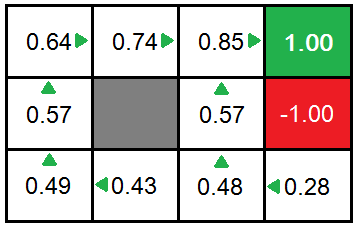
\includegraphics{img/policy.png}}
  \caption{Problém představuje pole o velikosti 12 polí (z nichž šedé je nedosažitelné), 4 směry možnosti chůze a dva koncové stavy s odměnami ohodnocenými -1 a 1. Problém je stochastický, přechod ze stavu do následníka se provede dle své pravděpodobnosti v přechodové funkci. Již po 5 iteracích je vidět optimální strategie, reprezentovaná šipkou směru (agent začíná v levém spodním rohu), vypočtena pomocí hodnoty $V_{5}$ každého pole.}
  \label{img:policy}
\end{center}
\end{figure}

MDP lze též reprezentovat prohledávacím stromem, viz obrázek \ref{img:mdptree}, který se velmi podobá Expectimaxu avšak jak již bylo řečeno není potřeba rekurze, pouze se iterativně vyhodnocuje nová vrstva $V_{k+1}$.
\newpage

\begin{figure}[ht]
\begin{center}
  \scalebox{0.8}{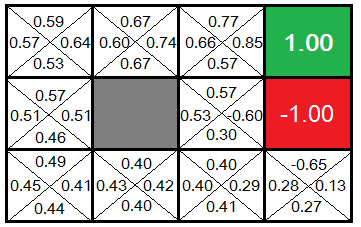
\includegraphics{img/qvallls.png}}
  \caption{Ukázka Q-hodnot pro předešlý grid-world problém (po 5. iteraci). Q-hodnoty se počítají pro každou možnou akci ze stavu do následníka, proto jsou pro jedno políčko na hracím plánu 4 pro každý směr, kam může agent jít.}
  \label{img:qvals}
\end{center}
\end{figure}

\begin{figure}[ht]
\begin{center}
  \scalebox{0.75}{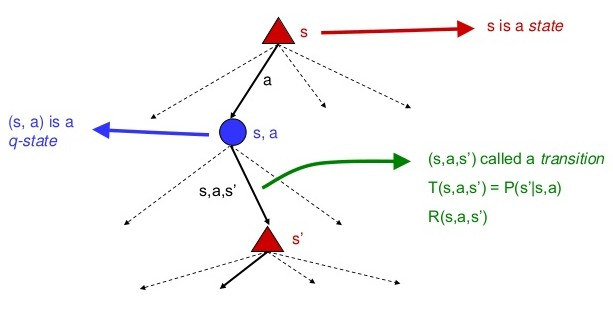
\includegraphics{img/mdptree.jpg}}
  \caption{Na obrázku lze vidět analogii MDP Value Iteration k Expectimaxu \cite{RLIntro}.}
  \label{img:mdptree}
\end{center}
\end{figure}
\newpage
\section{Strojové učení}
\label{sec:rl}
Další důležitou vlastností agenta bude schopnost \textit{učit se} \cite{RLIntro}. Agent se učí na pozorovaných výsledcích svých akcí, tzv. \textbf{vzorky} $(s,a,s^\prime,r)$, kde $r$ je odměna nového stavu. Stále se jedná o MDP, avšak největší rozdíl zde nastává v tom, že \textbf{není známá} odměnová funkci $R$, ani přechodová funkci $T$. Agent (viz obrázek \ref{img:learningagent}) se tedy musí metodou \textit{pokus-omyl} \textbf{naučit} tyto hodnoty modelu.

\begin{figure}[!htbp]
\begin{center}
  \scalebox{0.5}{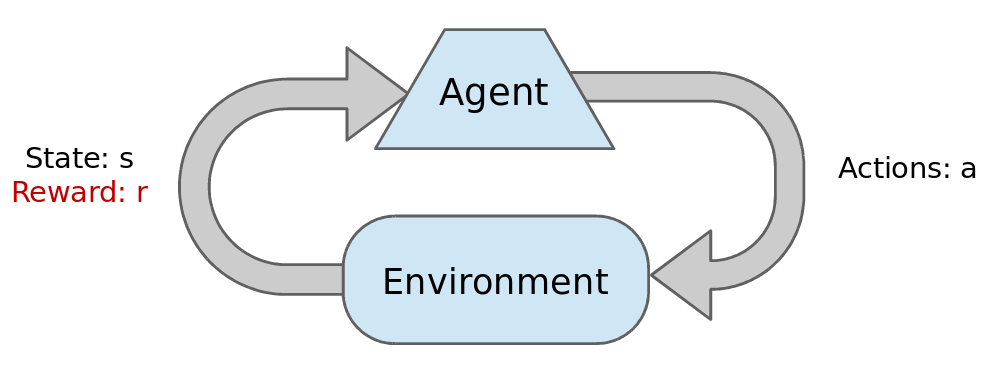
\includegraphics{img/learningagent.png}}
  \caption{Agent využívající strojové učení.}
  \label{img:learningagent}
\end{center}
\end{figure}

Metody strojového učení se dělí dle \textbf{závislosti na modelu} \cite{RLIntro} \cite{reifreview}:
\begin{itemize}
\item (\textit{model-based}) metoda chce empiricky vytvořit model, který již lze řešit pomocí MDP -- to se děje na základě průběžného výpočtu očekávaného užitku: 
\begin{enumerate}
\item Spočítej všechny výsledky/vzorky $s^\prime$ pro každý pár $(s,a)$.
\item Spočítej odhad okamžitého užitku, tedy odhad přechodové funkce $\hat{T}(s,a,s^\prime)$.
\item Odhadni odměnovou funkci $\hat{R}(s,a,s^\prime)$ na základě objevených odměn stavů.
\end{enumerate}
\item (\textit{model-free}) metoda model nepotřebuje, stačí posbírat vzorky, protože \textit{rozdělení pravděpodobnosti} pro daný vzorek určuje jeho výskyt (není potřeba počítat očekávaný užitek). Dále se budeme zabývat těmito metodami.
\end{itemize}

Dalším dělicím kritériem je \textbf{řízení akcí}:
\begin{itemize}
  \item \textit{pasivní metody} -- je daná statická strategie $\pi(s)$, kterou se agent pevně řídí a získává z ní vzorky, ze kterých se učí hodnoty stavů $V(s^\prime)$ pro daný stav $s$.
  \newline
  Ukázka postupu metody přímého vyhodnocení (\textbf{direct evaluation} \cite{berkeley}):
  \begin{enumerate}
    \item Následuj $\pi$.
    \item Pro každý navštívený stav vypočti sumu koeficientem $\gamma$ budoucích snížených hodnot.
    \item Spočítej průměr sumy.
  \end{enumerate}
  Není potřeba $T$ ani $R$, avšak je zde přílišná abstrakce (plýtvání informací) a vyhodnocení stavů díky tomu má příliš velkou časovou náročnost.
  \newline
  Další možností je \textbf{Time-Difference value learning} \cite{RLIntro}, dále TD učení, které se místo vyhodnocování hodnoty Value iteration (a nakonec teprve získání výsledné strategie) snaží vyhodnotit přímo nové strategie na základě hodnot (\textbf{Policy iteration}). Vyhodnocení probíhá \textit{po každé akci}, protože nelze zaručit, že se strategie bude vracet znovu do již vyhodnoceného stavu, aby opět přehodnotila svou hodnotu \cite{RLpaper}.
  \newline
  Ukázka postupu \textbf{TD učení}:
  \begin{enumerate}
    \item Následuj $\pi$.
    \item Aktualizuj $V(s)$ pokaždé, když narazíš na přechod pro vzorek $(s,a,s^\prime,r)$. \textbf{Aktualizace} (\textit{update}), spočívá v tom, že se vezme aktuální hodnota stavu a přičte se k ní o koeficient $\alpha$ zmenšený rozdíl mezi očekávaným stavem a reálným vzorkem. $\alpha$ reguluje fakt, že nové odměny budou mít větší váhu než staré.
    \begin{eqnarray}
    \textrm{Vzorek $V(s)$} &\textrm{:}& \quad vzorek = R(s,\pi(s),s^\prime)+\gamma V^\pi(s^\prime) \\
    \textrm{Update $V(s)$} &\textrm{:}& \quad V^\pi(s) \leftarrow  V^\pi(s) + \alpha(vzorek - V^\pi(s))
    \end{eqnarray}
  \end{enumerate}
  TD učení je pasivní metoda, která je schopna získat ohodnocení hodnot V, avšak není schopna aktivně přeměnit hodnoty na novou strategii $\pi(s)$ dle rovnic MDP pro Policy iteration (viz obrázek \ref{img:policyeval} \cite{berkeley}):
  \begin{eqnarray}
  \pi(s) &=& arg \max_a Q(s,a) \\
  Q(s,a) &=& \sum_{s^\prime}T(s,a,s^\prime) \left[R(s,a,s^\prime)+\gamma V(s^\prime) \right]
  \end{eqnarray}
  Problém je opět chybějící přechodová a odměnová funkce ($T,R$), to řeší až \textit{aktivní metody} strojového učení.

  \begin{figure}[!htbp]
  \begin{center}
    \scalebox{0.5}{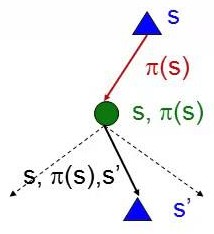
\includegraphics{img/policyeval.jpg}}
    \caption{Policy iteration metoda s potřebnými proměnnými (pomocí strategie $\pi$(s) se dostávám ze stavu $s$ do jeho následníka $(s^\prime)$).}
    \label{img:policyeval}
  \end{center}
  \end{figure}

  \item \textit{aktivní metody} -- je dána statická strategie $\pi(s)$, ale agent provádí vlastní akce a získává z nich vzorky, ze kterých se učí optimální strategie a hodnoty stavů $V(s^\prime)$. Mezi aktivní metody patří \textbf{Q-Learning}.
\end{itemize}

\subsection*{Q-Learning}
Dosud se primárně vycházelo z V-hodnot, avšak Q-Learning je založen na vyhodnocování posloupností akcí do nových stavů, tedy na využití Q-hodnot. Jediné, co je tedy potřeba vědět je aktuální stav a jeho možné akce \cite{RLIntro}:
\begin{align}
vzorek = \left [ R(s,a,s^\prime)+\gamma \max_{a^\prime}Q_{k}(s^\prime,a^\prime) \right]
\end{align}
Následně se provede aktualizace (update) TD učení, kde $\alpha$ nyní představuje rychlost učení (\textit{learning rate}):
\begin{align}
 Q(s,a) \leftarrow  Q(s,a) + \alpha(vzorek - Q(s,a))
\end{align}


\subsubsection{Q-Learning postup}
\label{teorie:qlearning}
\begin{enumerate}
  \item Navštiv nový uzel $s^\prime$.
  \item Ze vzorku $(s,a,s^\prime,r)$ vypočti novou hodnotu jeho odhadu $Q_{k+1}(s,a)$ jako:
  \newline
    průměr očekávaných užitků akcí stavu $T\:*\:$ (okamžitá odměna $+$ nejlepší možná Q-hodnota následníka $Q_{k}(s,a)$), tedy:
    \begin{align}
    Q_{k+1}(s,a) \leftarrow \sum_{s^\prime} T(s,a,s^\prime) \left[ R(s,a,s^\prime) + \gamma \max_{a^\prime} Q_k(s^\prime,a^\prime)\right]
    \end{align}
    Průměr $T$ a hodnoty odměn $R$ se postupně počítají na základě akcí (nejsou zpočátku známy), algoritmus se tedy blíží následující rovnici:
    \begin{align}
    Q(s,a) \approx r + \gamma \max_{a^\prime}Q(s^\prime,a^\prime)
    \end{align}
    kde $r$ je přímá odměna ze stavu \cite{imrewards}.
  \item proveď update TD učení (průměr odhadu vůči vzorku)
    \begin{align}
    \label{eq:qupdate}
     Q(s,a) \leftarrow  Q(s,a) + \alpha \left [ r + \gamma \max_{a^\prime} Q(s^\prime,a^\prime) \right]
    \end{align}
\end{enumerate}
Q-Learning konverguje k optimální strategii, i když následuje posloupnost neoptimálních akcí \cite{qlearnspringer}. Tento jev se nazývá \textit{off-policy learning} \cite{RLIntro}.
Jak ale agent vybírá, kterou akci provede, aby maximalizoval svůj užitek z tréninku? Je nutné zvolit dobrý poměr mezi zjišťováním terénu (\textit{exporation}) a využíváním již zjištěných aktuálních dobrých strategií (\textit{exploitation}) \cite{RLpaper}. Dobrý poměr lze řešit několika způsoby \cite{berkeley}:
\begin{itemize}
  \item Zavedením koeficientu $\varepsilon-greedy$ pro výběr náhodných akcí (vůči optimálním). Výhodné je ovšem koeficient časem zmenšovat, aby nedocházelo k nelogičnostem akcí.
  \item Využitím \textbf{explorační funkce}, která bere v potaz nejen budoucí užitek stavu $U$, ale i množství navštívění stavu $N$. Díky tomu se prozkoumají stavy, jejichž dosud zjištěná špatná hodnota ještě není úplně stabilní (málo výskytů). Funkce tedy snižuje důležitost opakujících se stavů a dává větší důraz na neprozkoumané stavy. Nakonec s tímto skončit, výsledná aktualizace hodnot (update) potom vypadá:
  \begin{align}
  Q(s,a) \leftarrow_\alpha R(s,a,s^\prime) + \gamma \max_{a^\prime} f(Q(s^\prime,a^\prime),N(s^\prime,a^\prime))\
  \end{align}
  Update se následně propaguje dál.
\end{itemize}
Novým pojmem pro metody posilovaného učení je \textbf{lítost} (\textit{regret}) jako míra toho, kolik agenta stály všechny chyby během tréninku (rozdíl mezi očekávanými odměnami a optimálními odměnami). Je snaha tuto co nejvíce míru minimalizovat (optimálně se i učit optimální řešení daného problému).

\subsection*{Approximační Q-Learning}
\label{sec:qlearning}
Zatímco základní Q-Learning pomohl zbavit se zbytečného přepočítávání hodnot, stále je potřeba si neustále udržovat tabulku všech Q-hodnot pro každou kombinaci stavu a akce. Pro složitou úlohu jakou je Ms. Pacman je tato velká prostorová složitost stavového prostoru stále nevhodná. Z toho důvodu je potřeba \textbf{generalizovat}: naučit se Q-hodnoty malého množství tréninkových stavů a hodnoty generalizovat na podobných situacích. To je důležitá myšlenka metody aproximační Q-Learning a potažmo i strojového učení \cite{RLAprox}:
\newline
popsání stavu pomocí vektoru vlastností (\textit{properties}), vlastosti jsou funkce ze stavů do reálných čísel (např. 0, 1), které zachycují důležité vlastnosti stavu. Následně lze tyto vlastnosti ohonodnotit \textbf{váhou} (\textit{weight}) a sesavit lineární rovnice \cite{RLAprox}:
\begin{eqnarray}
V(s) &=& w_1f_1(s) + w_2f_2(s) + \dots + w_nf_n(s) \\
Q(s,a) &=& w_1f_1(s,a) + w_2f_2(s,a) + \dots + w_nf_n(s,a)
\end{eqnarray}
Nevýhoda takové generalizace je ale fakt, že je potřeba stanovit co nejlepší vektor vlastností tak, aby se hodnoty rozdílných stavů nepodobaly.
\subsubsection{Aproximační Q-Learning postup}
\label{teorie:approxq}
\begin{enumerate}
  \item Navštiv nový uzel a ze vzorku $(s,a,s^\prime,r)$ vypočti rozdíl odhadu Q-hodnoty vůči vzorku:
    \begin{align}
	\label{rov:approxq1}
     rozdil = \left [ r + \gamma \max_{a^\prime}Q(s^\prime,a^\prime) \right]  - Q(s,a) 
    \end{align}
  \item Udělej aktualizaci (update) TD učení (průměr odhadu vůči vzorku)
    \begin{align}
	\label{rov:approxq2}
     Q(s,a) \leftarrow  Q(s,a) + \alpha \left [ r + \gamma \max_{a^\prime}Q(s^\prime,a^\prime) \right]
    \end{align}
  \item Následně místo updatu jedné Q-hodnoty (základní Q-Learning), aproximuj Q-hodnoty pomocí změny váhy $w_i$ vůči vektoru vlastností:
    \begin{align}
	\label{rov:approxq3}
    w_i(s) \leftarrow w_i + \alpha \left [ r + \gamma \max_{a^\prime}Q(s^\prime,a^\prime) - Q(s,a) \right] f_i(s,a)
    \end{align}
    kde:
    \begin{itemize}
      \item $\left [ r + \gamma \max_{a^\prime}Q(s^\prime,a^\prime)\right] $ reprezentuje cíl (maximální), kterého se snaží daný stav dosáhnout (nejlepší odhad Q-hodnoty následujícího stavu).
      \item $\left [ Q(s,a)\right]$ vzorek aktuálního stavu.
      \item $f_i(s,a)$ lineární funkce, jejíž rozdíl vzorků je aproximován\footnote{K aproximaci se používá obecná \textbf{Metoda nejmenších čtverců, tzv. lineární regrese}}, což napomáhá možnosti využití i nelineárních funkcí ve vektoru vlastností. Funkce reflektuje předpoklad odhadu Q-hodnoty následujícího stavu.\newline
      Zjednodušeně řečeno např. u Ms. Pacman: Pokud Ms. Pacman narazí do ducha, zvětší se váha vlastnosti situace ohrožení Ms. Pacman duchem. Pokud se tedy stane nějaká pozitivní akce, pozitivní váha zvětší hodnotu vlastnosti ve vektoru vlastností a naopak.
    \end{itemize}

\end{enumerate}

\chapter{Analýza a návrh}
\label{anavrh}
Tato kapitola se podílí na praktické části práce a to především praktické analýze problematiky Ms. Pacman (první část \ref{analyza}) a návrhu \textbf{chování agentů} (druhá část \ref{navrh}).

\section{Analýza}
\label{analyza}
\subsection*{O hře a důvod jejího výběru}
\textit{Ms. Pacman} je arkádová hra z roku 1982, která vylepšuje původní koncept hry Pacman. Hra je obohacena o nový design hlavní postavy, mapy a především implementuje lepší umělou inteligenci nepřátel. Hlavní postavou ovládanou hráčem je nyní Ms. Pacman, nepřátelé zůstávají v podobě 4 barevných duchů. Cílem hry je dosáhnout co největšího skóre pojídáním kuliček, duchů (časově omezené; po snězení speciální větší kuličky tzv. power-upu), nebo ovoce.
Zvýšení obtížnosti oproti Pacmanovi spočívá především v \textbf{opuštění deterministického chování duchů}, čímž pádem nelze předpovídat jejich chování. Tento fakt spolu se složitostí hry jsou hlavními faktory proč se na hru zaměřit z hlediska strojového učení. Ukázka původní verze hry je vidět na obrázku \ref{img:mspac}.

\subsection*{Pravidla}
Pro účely této práce se bere v potaz zjednodušení původní hry na vizuální demo tak, aby byla dobře vidět účinnost jednotlivých algoritmů a nebyly příliš vysoké nároky na výpočetní výkon. Demo není rozděleno na levely, odehrává se na zvolené mapě a je založeno na umělé inteligenci obou stran (Ms. Pacman vs 2 duchové). Cíl Ms. Pacman je maximalizovat skóre na aktuální mapě, zatímco cíl nepřátel je její skóre minimalizovat. Stochastické chování nepřátel je simulováno tak, aby co nejvíce odpovídalo svému vzoru (zdrojové kódy hry nejsou veřejné, tudíž nelze simulovat chování duchů naprosto stejně jako v originálu: chování duchů je tedy \textbf{náhodné}, avšak duchové dodržují např. následující pravidlo: nemohou jít zpět, pouze se otočit na křižovatce např. o 90 stupňů.). Duchové se snaží chytit a zabít Ms. Pacman. Pokud se jim to povede, hra končí (skóre - 500 bodů). Skóre Ms. Pacman se navyšuje jezením jídla (skóre + 10bodů za jednu kuličku), power-upů a následným jezením duchů (skóre + 200 bodů za každého ducha) po omezený čas trvání power-upu. Bonusová ovoce se neberou v potaz. Skóre se snižuje po dobu chození Ms. Pacman po bludišti bez jezení ovoce/duchů (každé takové kolo skóre - 1 bodů). Mapy se též liší, jsou menší a obsahují pro umělou inteligenci Ms. Pacman problémová zákoutí, jako větší neohraničené plochy, stísněný prostor atp. Ms. Pacman a duchové mají stejnou rychlost. Tato zjednodušení slouží především ke snížení vypočetní náročnosti algorimů na běžně dostupný hardware.

\begin{figure}[!htbp]
\begin{center}
  \scalebox{0.9}{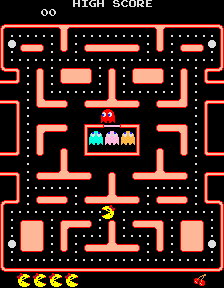
\includegraphics{img/Mspacman.png}}
  \caption{Screenshot 1. levelu originální verze Ms. Pacman.}
  \label{img:mspac}
\end{center}
\end{figure}

\subsection*{Klasifikace dema Ms. Pacman z hlediska Teorie her}
Ms. Pacman je hra, tzn. strategická interakce mezi 2 a více hráči, kteří chtějí dosáhnout optimálního výsledku ve hře.
Vizuální demo Ms. Pacman lze specifikovat podle několika kritérií:
\begin{itemize}
  \item \textbf{dle informovanosti hráče o hře:} \textit{hra s neúplnou informací} (\textit{game with uncertainty}) -- duchové mají stochastické chování,
  \item \textbf{dle počtu tahů:} \textit{hra strategická} – hráči provádějí souběžná rozhodnutí,
  \item \textbf{dle míry konkurence/typu výhry:} \textit{hra s nulovým součtem} (\textit{zero-sum game})  -- jeden hráč maximalizuje svou výhru a druhý minimalizuje ztrátu (míra výhry jednoho značí míru prohry druhého hráče),
  \item \textbf{dle počtu hráčů:} Ms. Pacman je maximizér a 2 duchové jsou minimizéři,
  \item \textbf{dle komunikace hráčů:} \textit{nekooperativní hra} – Ms. Pacman a duchové spolu nekomunikují a souběžně hrají proti sobě (striktně kompetitivní hra),
  \item \textbf{dle zdrojů:} \textit{antagonistický konflikt} – Ms. Pacman a duchové sdílí jedno pevné maximální skóre dle herního plánu: \textit{gridworld game} – vše probíhá diskrétně, po polích na mřížce v herním bludišti, jež mohou nabývat více stavů: prázdná cesta, zeď, prázdná cesta s hráčem, cesta s kuličkou, cesta s power-upem.
\end{itemize}

\section{Návrh}
\label{navrh}
Po nastudování teorie a analýze chování nepřátel ve hře (duchů) je důležité jasně poupravit cíle práce: budou se porovnávat nejen metody Minimax a Alfa-Beta Řezy s učícím agentem, ale především také Expectimax, který bere v potaz stochastičnost akcí duchů. Tyto algoritmy se budou dále v textu označovat jako \textit{základní algoritmy}.
\newline
Pro výpočet vzdáleností bude použita tzv. \textit{manhattonovská metrika} \cite{manhattanDist} jako standard pro gridworld problematiku, kde figuruje mřížka a 4 směry pohybu agenta (Lze vidět na obrázku \ref{img:manhattanDist}). Tato vzdálenost je měřena jako suma rozdílu absolutních vzdáleností koordinát dvou bodů $\left|x1-x2\right|+\left|y1-y2\right|$.

\begin{figure}[!htbp]
\begin{center}
  \scalebox{0.08}{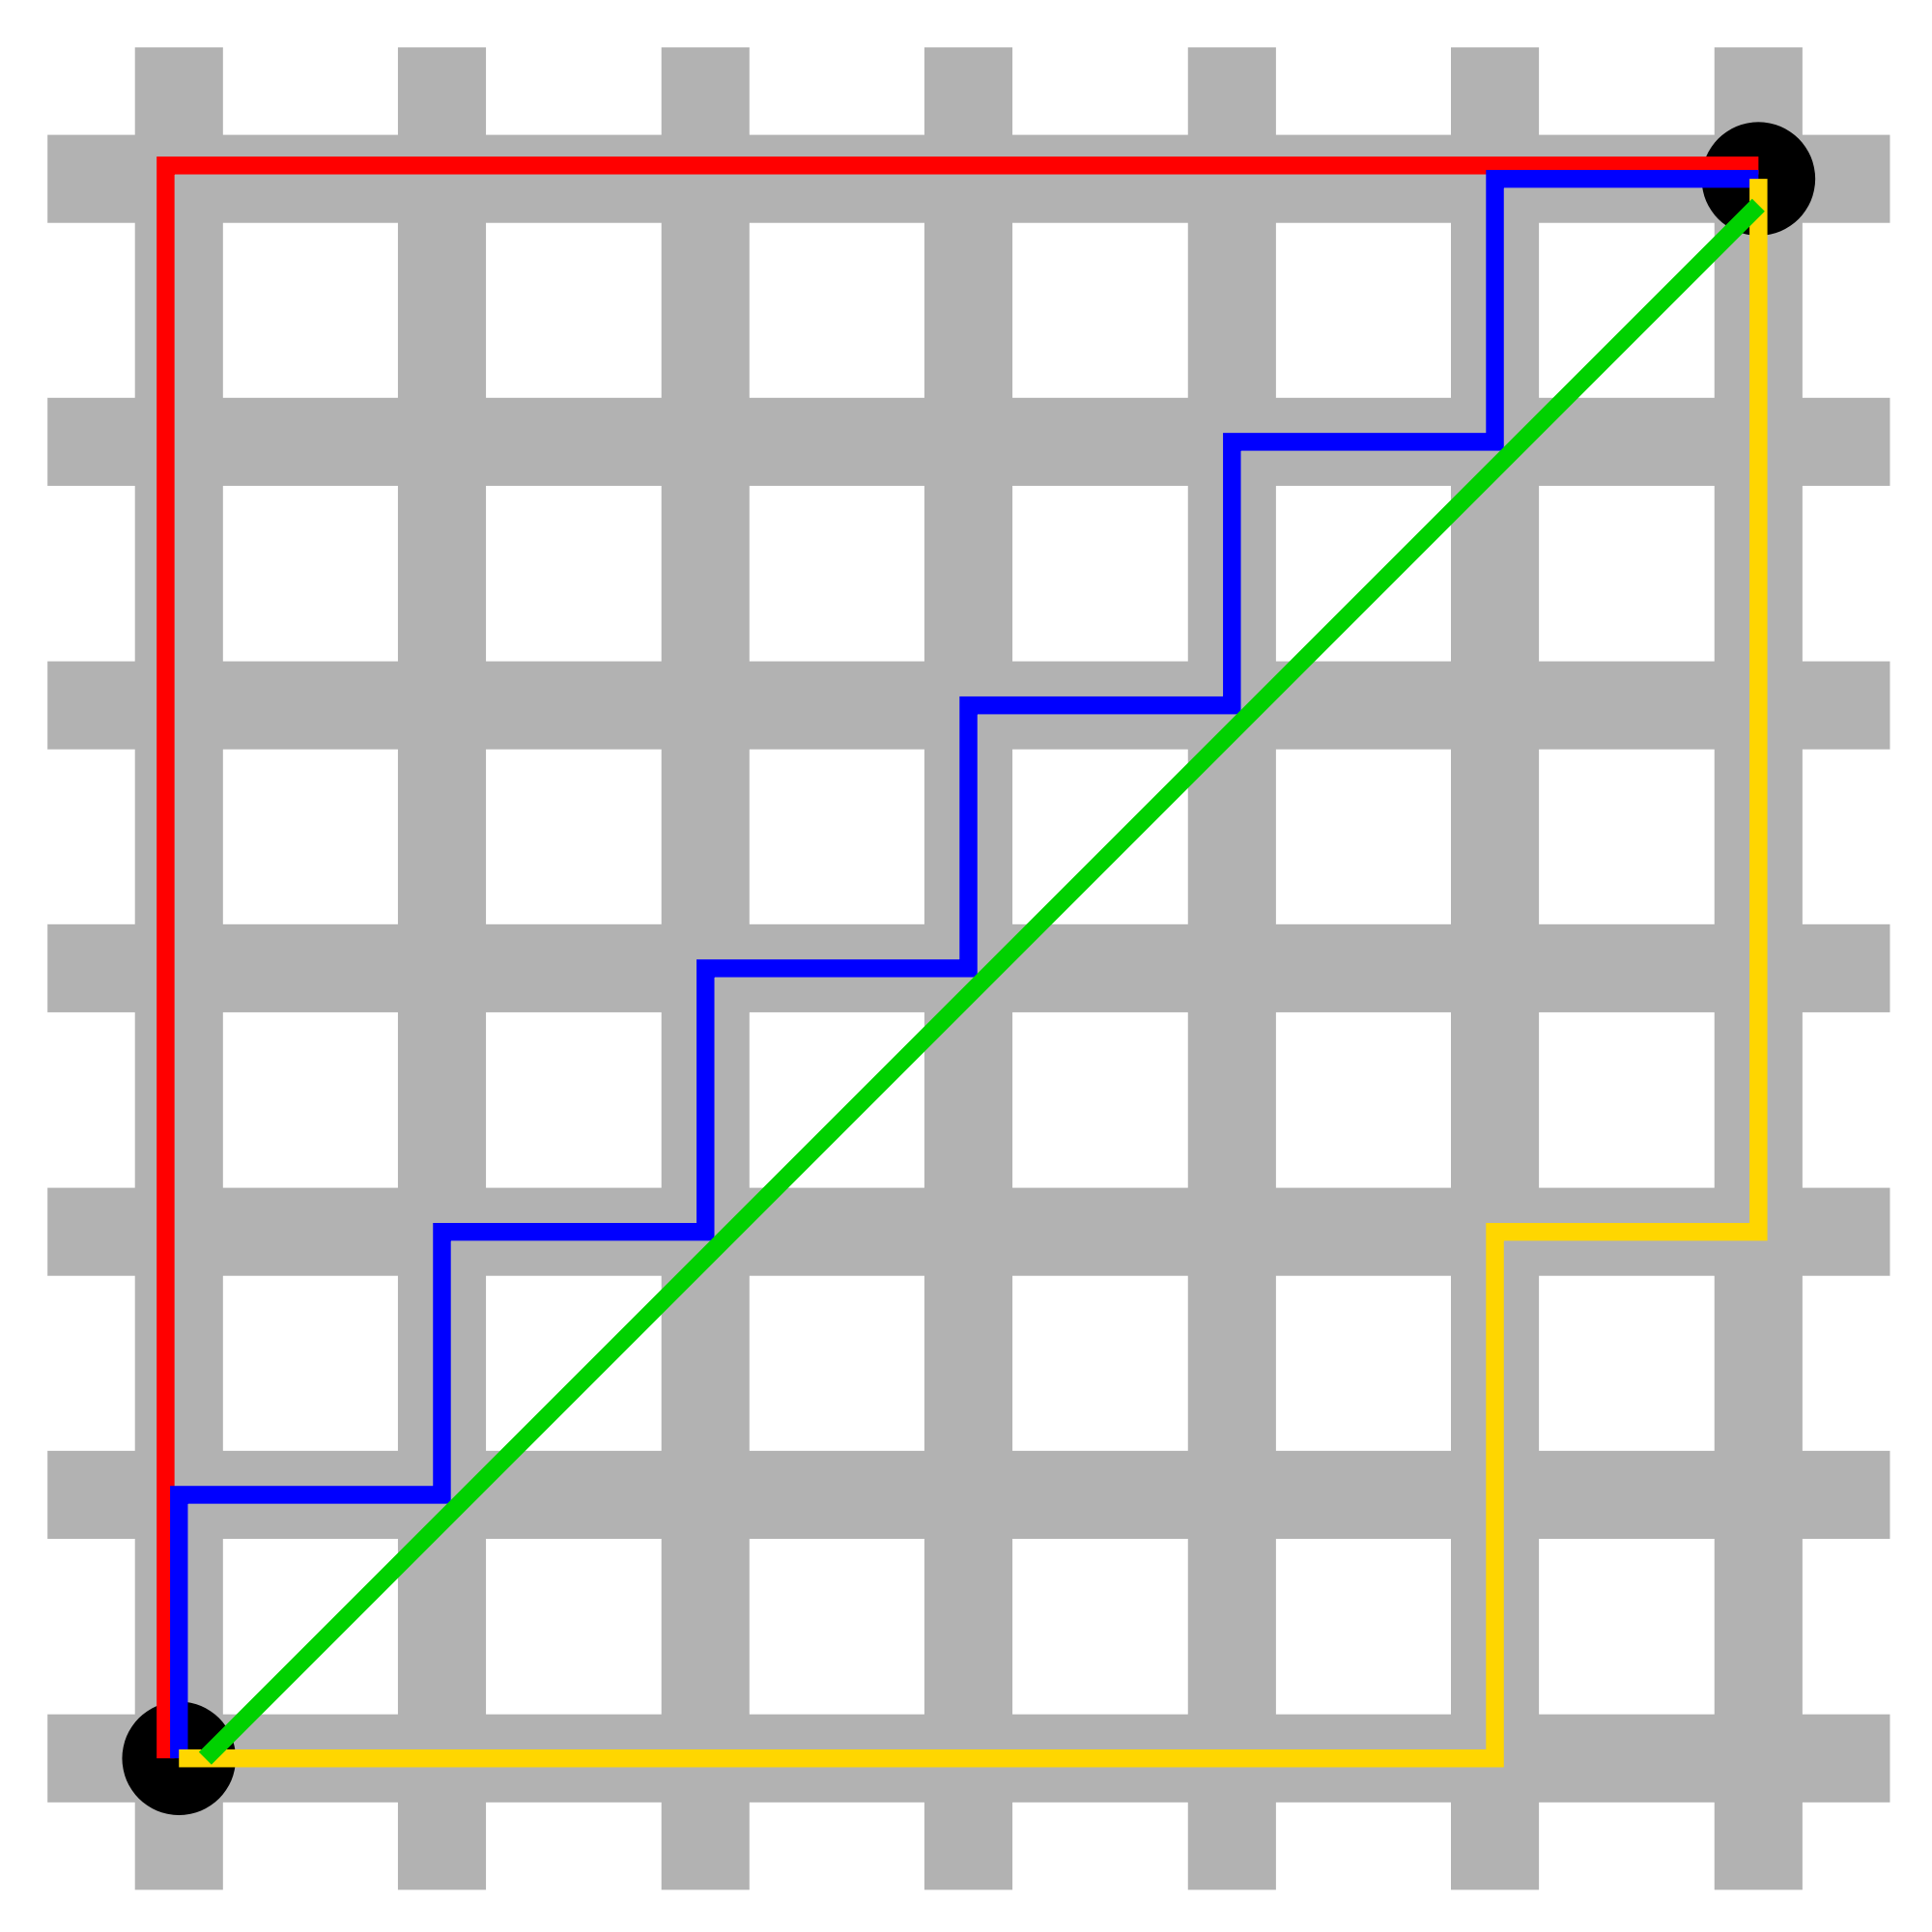
\includegraphics{img/manhattan.png}}
  \caption{Červená, modrá i žlutá čára reprezentují stejnou manhattonskou vzdálenost o velikosti 12 (narozdíl od Euklidovské vzdálenosti reprezentované zelenou čárou.)}
  \label{img:manhattanDist}
\end{center}
\end{figure}

\subsection*{Minimax, AlfaBeta řezy}
\label{navrh:minabmaxy}
Pro základní algoritmy bylo nutné vzít v potaz větší počet minimalizujících nepřátel, kteří se v každém tahu dané hloubky střídají s maximalizující Ms. Pacman, viz obrázek \ref{img:playersminimax}. Alfabeta i Minimax budou využívat vyhodnocovací funkci založenou na skóre následníka stavu ve hře. Algoritmy vyhodnocují stavy až do stanové hloubky/terminální uzlu a následně vrátí nejlepší možnou akci pro svého maximalizačního agenta Ms. Pacman.

\begin{figure}[!htbp]
\begin{center}
  \scalebox{0.3}{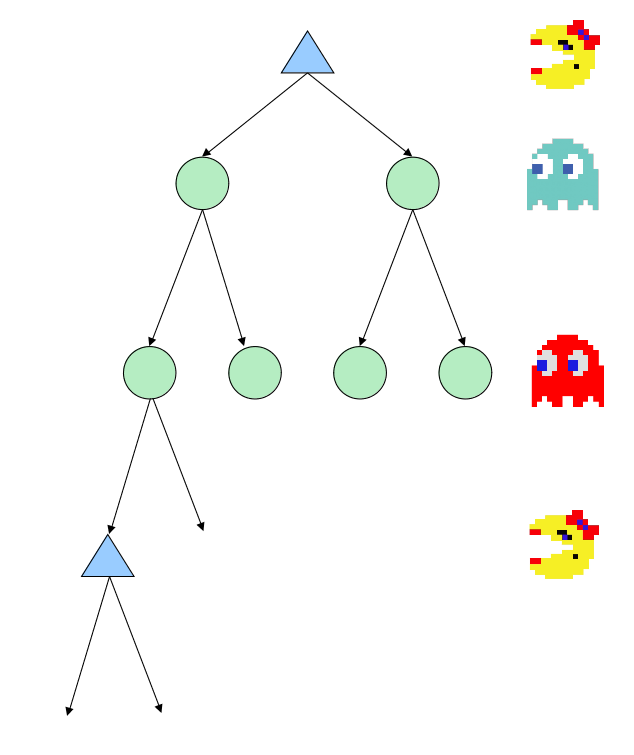
\includegraphics{img/playersminimax.png}}
  \caption{Ukázka střídání hráčů na stromu algoritmu Minimax.}
  \label{img:playersminimax}
\end{center}
\end{figure}
\newpage
\subsection*{Expectimax a lepší ohodnocovací funkce}
\label{navrh:expectimax}
Jelikož Expectimax průměruje hodnoty následníků ve svých uzlech náhodnosti \textit{chance node}, bere tedy v potaz hodnoty všech stavů (ne jen těch nejlepších a nejhorších, jak tomu bylo doposud). Proto bude pro tohoto agenta bude naimplementována kvalitnější vyhodnocovací funkce, která by měla společně s algoritmem dosáhnout lepšího skóre než u předchozích agentů vzhledem ke stochastičnosti pohybu nepřátel. Funkce bere v potaz nejen herní skóre následníka, ale také další součásti stavu hry (vzdálenosti jídla, duchů, power-upů atp. Tato funkce by se dala do budoucna vylepšit o algoritmy prohledávání stavového prostoru jako \textit{BFS}, \textit{DFS}\footnote{\textit{BFS} = slépé prohledávání do šířky, \textit{DFS} = slepé prohledávání do hloubky; tyto a další metody popisuje \cite{AI1}}, atp. tak, aby se dále brala v potaz například pozice stěn na herní desce. 
\newline
Samotný algoritmus Expectimax je (stejně jako Alpha Beta řezy) založený na algoritmu Minimax a je také z hlediska porovnání s pokročilými metodami umělé inteligence nejzajímavější, proto lze jako názornou ukázku uvést právě návrh jeho pseudokód \ref{alg:expectimax}. Algoritmus se dále bude muset provázat s \textbf{akcí}, jež má každý agent provést na základě vyhodnocené hodnoty svého uzlu.

\begin{algorithm}
\caption{\textbf{Expectimax} -- pseudokód vyhodnocování hodnot stavů, 1. část}
\label{alg:expectimax}
\begin{algorithmic}[1]

\Require stav hry
\Ensure užitek stavu
\Function{Expectimax}{stav}
  \If{terminální uzel}
    \State \Return $\text{\Call{vyhodnocovaciFunkce}{stav}}$  \Comment{navrať užitek stavu}
  \EndIf
  \If{další agent == MAX}
    \State \Return $\text{\Call{maxNode}{stav}}$  \Comment{vrstva Ms. Pacman = maximalizační}
  \EndIf
  \If{další agent == EXP}
    \State \Return $\text{\Call{chanceNode}{stav}}$  \Comment{vstva nepřátel = odhad tahu}
  \EndIf
\EndFunction
\algrule
\Require stav hry
\Ensure hodnota uzlu pro Ms. Pacman
\Function{maxNode}{stav}
    \State hodnota = $-\infty$
    \ForAll{následníci stavu}
    \State tmp = $\text{\Call{Expectimax}{následník}}$
    \If{tmp $>$ hodnota} \Comment{získej nejlepší možnou hodnotu pro Ms. Pacman}
        \State hodnota = tmp
      \EndIf
    \EndFor 
    \State \Return hodnota
\EndFunction
%\algstore{alg:expectimax}
%\end{algorithmic}
%\end{algorithm}
%\newpage
%\begin{algorithm}
%\caption{\textbf{Expectimax} -- pseudokód vyhodnocování hodnot stavů, 2. část}
%\label{alg:expectimax}
%\begin{algorithmic}[1]
%\algrestore{alg:expectimax}
\algrule
\Require stav hry
\Ensure hodnota uzlu pro nepřítele
\Function{chanceNode}{stav}
    \State hodnota = 0
    \ForAll{následníci stavu}  
    \State // pravděpodobnost výskytu následníka  
    \State p = $\text{\Call{pravděpodobnost}{stav,následník}}$
    \State hodnota += p * $\text{\Call{Expectimax}{následník}}$
    \EndFor
    \State \Return hodnota \Comment{navrať průměrnou hodnotu všech následníků}
\EndFunction

\end{algorithmic}
\end{algorithm}
\newpage

\subsection*{Provedení chování pokročilých agentů}
Všichni následující agenti průběžně (na základě zjištěných Q-hodnot ke každému poli herní desky) vyhodnocují, jakou akci mají z daného pole hrací desky nejlépe provést = strategie $\pi^*$ (\textit{policy}). Chování agentů, neboli \textbf{provedení strategie} (posloupnost akcí na desce) se bude demonstrovat v rámci tzv. \textbf{epizod} (jedna epizoda = jeden pokus agenta o provedení zjištěné optimální strategie). Samotný rozdíl v návrhu vyhodnocování zjištěných {V-hodnot} a Q-hodnot popisují jednotlivé sekce každého agenta (Value Iteration agent \ref{navrh:valiteragent}, Q-Learning agent \ref{navrh:qlearnagent}, Aproximační Q-Learning agent \ref{navrh:approxqlearnagent}). Zjednodušený pseudokód návrhu vyhodnocování chování následujících agentů lze vidět na algoritmu \ref{alg:behaviour}. Jak lze vidět, výsledné chování agenta je prováděno podobně, avšak u Q-Learningových agentů se na základě zjištěných okamžitých odměn provede \textbf{aktualizace Q-hodnot} a také se navíc bude dále rozlišovat, zda je agent v tréninku (= provádí epizody tréninku, tedy strategie v rámci \textit{exploration} může být i náhodná), či pouze provádí zjištěnou optimální strategii (= provádí chování během epizod stejně jako Value Iteration agent).

\begin{algorithm}
\caption{\textbf{Pokročilí agenti} -- provedení strategie}
\label{alg:behaviour}
\begin{algorithmic}[1]

\Require herni deska, agent, počet epizod
\Procedure{behaviour}{deska,agent,maxEpizod}
  \For{i = 0; i $<$ maxEpizod; i++}
    stav = počáteční stav
    \State{terminální stav nemá žádné připustné akce}
    \While{stav != terminální stav}
      \State akce = agent.$\text{\Call{getPolicy}{stav}}$ \Comment{získej strategii}
      \State // proveď strategii pro stav, získej odměnu
      \State (následník,odměna) = deska.$\text{\Call{doPolicy}{stav}}$
      \State // pokud učící agent trénuje (neprovádí pouze zjištěnou strategii)
      \If{agent.typ == QLearnAgent \textbf{or} agent.typ == ApproxQLearnAgent}
        \If{agent.trenink}
          \State // aktualizuj novou hodnotu pro pár (stav,akce)
          \State agent.$\text{\Call{QUpdate}{stav,akce,následník,odměna}}$
        \EndIf
      \EndIf
      \State stav = následník
    \EndWhile
  \EndFor
\EndProcedure

\end{algorithmic}
\end{algorithm}

\subsection*{Value Iteration agent}
\label{navrh:valiteragent}
Tento agent je \textbf{pasivní plánovací agent} -- provede veškeré své výpočty odhadů hodnot pomocí daného modelu světa a naplánuje si po každé iteraci akci pro danou hodnotu. Přepočet odhadů V-hodnot probíhá vždy do určitého stanoveného počtu $k$ iterací (podobné jako hloubka, agent by měl provést $k$-kroků výpočtu odhadů V-hodnot), nebo dokud metoda nekonverguje. Teprve po tomto provedení přepočtu hodnot je k dispozici optimální strategie pro herní desku a přichází doba provedení chování agenta ve formě epizod.

Velký vliv na průběh tohoto a následujících algoritmů má koeficient odměny $\gamma$ -- čím je koeficient menší, tím se vyhodnocení hodnot zpomaluje a důkladněji se tak prozkoumá více hodnot (výsledné vyhodnocení posloupnosti akcí může například trvat déle vyhodnotit, ale pravděpodobnost optimality výsledné strategie bude větší).

Dalším důležitou konstantou je odměna po každém agentově kroku (\textit{living reward}), tedy ohodnocení pohybu z jednoho neterminálního stavu do druhého. Odměna může být i záporná -- čím je menší, tím rychleji se agent snaží najít terminální uzel a skončit tak hru/problém. 

Poslední důležitý vliv na algoritmus má náhodnost pohybu agenta (\textit{noise}, která modeluje stochastičnost akce, tedy pravděpodobnost, že se daná akce provede -- ovlivňuje, jak často agent riskuje. \textit{Living reward} a \textit{noise} budou spravovány herní deskou.
\newline
Algoritmus bude implementován dle rovnic z teoretické sekce \ref{teorie:valiterq}. Agent tedy potřebuje (mj.) pro každou iteraci $k$ průběžně ukládat vektor \textbf{vHodnoty} všech stavů ($V\left[k\right]$), který vyhodnocuje své hodnoty pro stav na základě Q-hodnot stavu (odhady nejlepších akcí ze stavu do následníka dle rovnice \ref{eq:valiter22}). Dále je potřeba především \textbf{model} definující přechodovou a odměnovou funkci. Model musí být sestaven na základě stavů herní desky ještě před začátkem samotné metody. Pro ukázku si lze uvést vyhodnocení Q-hodnoty stavu na základě modelu v pseudokódu \ref{alg:valiterq}:
 
\begin{algorithm}
\caption{\textbf{Value Iteration} -- pseudokód získání Q-hodnot}
\label{alg:valiterq}
\begin{algorithmic}[1]
\Require model,aktuální stav,vybraná akce, gamma, vektor V-Hodnot (vHodnoty)
\State qHodnota = 0.0
\ForAll{naslednici z modelu}
  \State{pravděpodobnost přechodu z jednoho stavu do druhého}  
  \State p = model.$\text{\Call{prechodovaFunkce}{stav,akce,naslednik}}$
  \State{získaná odměna přechodu}
  \State r = model.$\text{\Call{odmenovaFunkce}{stav,akce,naslednik}}$
  \State qHodnota += p * ( r + gamma * vHodnoty[naslednik])
\EndFor
\Ensure Q-Hodnota(stav,akce) (qHodnota)
\end{algorithmic}
\end{algorithm}
\newpage

\subsection*{Q-Learning agent}
\label{navrh:qlearnagent}
Zatímco metoda Value Iteration má k dispozici Q-Hodnoty z modelu, z nichž si sestavuje vektor V-Hodnot, Q-Learning agent se během tréninku \textbf{aktivně učí} Q-hodnoty akcí (jejich pravděpodobnosti výskytu i odměny) a tím průběžně vytváří vlastní odhady Q-hodnot. Na výpočet Q-hodnot během tréninku má kromě již uvedených parametrů (z předchozí sekce) velký vliv parametr $\epsilon-greedy$, který určuje určuje pravděpodobnost, zda se má provést optimální (pravděpodobnost $1-\epsilon$), či náhodná akce (pravděpodobnost $\epsilon$) \textit{(exploitation/exploration ratio)}. Čím je tento parametr vyšší, tím pravděpodobněji se agent chová dle své akuální optimální akce. Dalším důležitým faktorem je $\alpha$, která ovlivňuje rychlost učení. Čím je větší alfa, tím víc se dává důraz na nové vzorky. Experimentální část práce \ref{exper} se také zaměřuje na co nejvhodnější stanovení těchto parametrů a jejich vliv na kvalitu výsledné umělé inteligence pro daný problém.
\newline
Hlavní náplní agenta je sestavit tabulku aktuálních odhadů Q-Hodnot ke všem párům (stav,akce). Tabulka se postupně zaplňuje a obnovuje novými $Q^*$-hodnotami zjišťovanými aktivně po provedení akce z jednoho stavu do svého následníka dle rovnic v sekci \ref{teorie:qlearning} (vyvoláno aktualizací hodnot).

Vyhodnocování a sestavování tabulky Q-Hodnot běhěm agentova tréninku lze vidět na pseudokódu inicializace a aktualizace hodnot \ref{alg:qlearn}, který návazuje na pseudokód \ref{alg:behaviour}. Aktualizace hodnot vychází přímo z rovnice \ref{eq:qupdate}).
\begin{algorithm}
\caption{\textbf{Q-Learning} -- pseudokód}
\label{alg:qlearn}
\begin{algorithmic}[1]
\Require herní deska, agent, počet Epizod, stavy, akce, tabulka Q-Hodnot qHodnoty
\Require globálně -- alfa, gamma, epsilon
\Procedure{QLearning}{deska,agent,maxEpizod,stavy,akce,qHodnoty}
  \ForAll{qHodnoty}
    \ForAll{pripustne akce}
      \State qHodnoty[stav,akce] = 0.0 \Comment{inicializace}
    \EndFor
  \EndFor
  \State // aktivně prováděj akce dle $\epsilon$ a updatuj qHodnoty
  \State $\text{\Call{behaviour}{deska,agent,maxEpizod}}$
\EndProcedure
\algrule
\Require stav, akce, naslednik, získaná odměna
\Require globálně -- alfa, gamma, epsilon, tabulka Q-Hodnot qHodnoty
\Procedure{QUpdate}{s,a,novýS,r}
  \State // získej odhad hodnoty budoucí optimální akce
  \State maxHodn = $\text{\Call{getValue}{novýS}}$
  \State // proveď aktualizaci (update) TD učení
  \State qHodnoty[s,a] +=  alfa * ((r + gamma * maxHodn) -- qHodnoty[s,a])
\EndProcedure
\end{algorithmic}
\end{algorithm}
\newpage

\subsection*{Aproximační Q-Learning agent}
\label{navrh:approxqlearnagent}
Pro vyhodnocování chování agenta není potřeba ukládat tabulku Q-hodnot pro každý pár (stav, akce), ale \textbf{váhy vlastností} a \textbf{vektor vlastností} (\textit{feature vector}), tedy vektor namapování dané vlastnosti na její aktuální hodnotu.
Vektor vlastností předpovídá odhad Q-hodnot jednotlivých párů $(stav,akce)$, které se budou využívat při vyhodnocení optimální strategie. Důležité je především korektě stanovit typy vlastností a jejich ohodnocení (podobně jako ohodnocovací funkce stavu):
\begin{itemize}
\item vzdálenost nejbližšího ducha a jeho stav,
\item vzdálenost nejbližší kuličky jídla,
\item vzdálenost nejbližšího power-upu,
\item počet zbývajícího jídla a power-upů na herní desce,
\item počet duchů,
\item pozice Ms. Pacman -- je v rohu?
\end{itemize}
Následně se stanoví návrh aproximační funkce vektoru na základě váhy každé vlastnosti a její funkční hodnoty, např.:
\begin{align}
Q(s,a) = w_{DUCH}f_{DUCH}(s,a) + w_{JIDLO}f_{JIDLO}(s,a) + \dots + w_{ROH}f_{ROH}(s,a)
\end{align}
kde 
\begin{itemize}
  \item $w$ je váha vlastnosti, $f$ je funkce vlastnosti,
  \item DUCH (reprezentuje vlastnost:) vzdálenost nejbližšího vystrašeného ducha (lze sníst),
  \item JIDLO vzdálenost nejbližší kuličky jídla,
  \item ROH zda je Ms. Pacman je v rohu.
\end{itemize}

Dále bude především potřeba nalézt \textbf{optimální strategii} během epizod tréninku pomocí \textit{(exploitation/exploration ratio)} a návrhu postupu metody Aproximační Q-Learning:
\begin{enumerate}
\item Aproximačně najdi model odhadů Q-hodnot během tréninku na základě hodnoty vlastnosti a její váhy (při novém přechodu proveď aktualizaci váh dle rovnice \ref{rov:approxq3}).
\item Předpokládej pouze Q-hodnoty akcí z daného stavu.
\item Opakuj předchozí body dokud nebude dost vzorků popř. neskončí trénink, jinak pokračuj na další bod.
\item Poměňuj váhy vlastností a testuj optimálnost nové strategie.
\end{enumerate}
Poměňování váh vlastností takto může \textbf{maximalizovat odměny} a dojít tak k lepší strategii, něž byla doposud použita.

\chapter{Realizace}
\label{realizace}
Tato kapitola popisuje praktickou část práce a především se zaměřuje na \textbf{implemetace různého chování agentů}.

\section{Zvolené prostředky}
Nejdříve bylo nutné si zvolit programovací jazyk, který by zvládl výpočetní náročnost problematiky vůči vykreslování grafického dema. Zpočátku byl zvolen jazyk \textit{Java} díky jeho vysoké míře abstrakce a intuitivnímu objektově zaměřenému přístupu jazyka. Během implementace se však narazilo na několik problémů: 
\begin{enumerate}
\item propojení herního prostředí s reprezentací jeho stavů pro spravné vyhodnocení umělou inteligencí + následné propojení stavů s MDP,
\item výpočetní náročnost algoritmů versus množství stavů ve hře,
\item snaha co nejvíce dodržet matematické vzorce z teorie,
\item názorné vykreslení výsledků složitějších algoritmů,
\item časová náročnost implementace logiky a GUI hry versus zaměření práce na umělou inteligenci.
\end{enumerate}
Nakonec po sérii experimentování s jazykem se kvůli zmíněným problémům přešlo k hledání náhradního řešení. Tím se stalo hledání aplikace, nebo frameworku, který řeší podobnou problematiku. Základem pro studii a experimentování s algoritmy nakonec posloužil pythonový framework od univerzity UC Berkeley \cite{pacmanProjects}, používaný v jejich výuce Úvod do umělé inteligence (kurz CS188) \cite{berkeley}. Hlavním důvodem zvolení frameworku tedy bylo především zaměření práce na experimentování s algoritmy umělé inteligence (oproti implementaci samotného jádra hry). Dalším důvodem volby je použití jazyka \textit{Python 2.7.5}, který též umožňuje objektový přístup, je dobře čitelný a nenáročný -- nejen díky těmto kladům se dají dobře pochopit vlastnosti a propojení jednotlivých objektů frameworku. Posledním faktorem volby byl také samotný nápad zaměření této práce -- přednášky kurzu UC Berkeley napomáhaly při analýze teorie pro tuto práci. Framework primárně posloužil jako prostředek pro realizaci a srovnání algoritmů a jejich názorné zobrazení výsledků.
Pro účely této práce budou v následující sekcích popsány nejdůležitější části aplikace, detailní popis implementace frameworku a vlastních algoritmů lze najít v komentářích v kódu. Ovladání frameworku lze nalézt v příloze \ref{priloha:manual}.

\section{Framework a reprezentace stavu hry}
Pro všechny algoritmy je nejdůležitější částí frameworku objekt \texttt{GameState} reprezentující \textbf{stav hry}, který lze najít ve spustitelném souboru \texttt{pacman.py}. Tento soubor a soubor \texttt{game.py} tvoří samotné jádro frameworku pro problematiku Ms. Pacman -- definují základní chování agentů, možné akce apod.
Dalším důležitým spustitelným souborem pro problematiku názornějšího zobrazení V a Q hodnot ve formě několika gridworld problémů je \texttt{gridworld.py}.
GameState dále pracuje s objekty \texttt{PacmanRules} a \texttt{GhostRules}, které zajišťují logiku přípustných akcí pro svého agenta(agenty).
Tento základní objekt tedy obsahuje:
\begin{itemize}
\item pozice Ms. Pacman a duchů,
\item pozice zbývajícího jídla v mřížce,
\item pozice zbývajících power-upů v mřížce,
\item pozice zdí v mřížce,
\item počet duchů,
\item možné akce, jež může daný agent provést z aktuálního stavu,
\item schopnost provést akci a vytvořit tak svého následníka (opět objekt \texttt{GameState}).
\end{itemize}
Každý agent dědí ze základního objektu \texttt{Agent} povinnou metodu \texttt{getAction} (zavazuje agenta přijmout objekt \texttt{GameSate} a vrátit na něj reakci v podobě akce) a proměnnou \texttt{index} definující index agenta (Ms. Pacman má tradičně index = 0).
Implementace vlastního chování konkrétního typu agenta je již definována v jeho vlastním objektu (jako override). Např. \texttt{AlphaBetaAgent} přetěžuje metodu \texttt{getAction} jako algoritmus Alfa-Beta řezy atp.

\section{Reflexivní agent a jeho ohodnocovací funkce}
Pro další srovnání s algoritmy byl implementován tento základní typ neadversárního reflexivního agenta \texttt{ReflexAgent}. Agent pouze vnímá aktuální stav hry (hloubka = 1) a jeho ohodnocovací funkce vyhodnocuje stav hry na základě informací o celém stavu hry. Chování reflexivního agenta je založeno na jednoduché ohodnocovací funkci svých následníků: agent se nejdříve podívá na ohodnocení stavů, tedy jejich užitek, po podniknutí všech přípustných \textit{Akcí} (jít vlevo, vpravo, nahoru, dolů, zastavit se) a následně pseudonáhodně vybere výslednou akci stavu s nejlepším ohodnocením.
\textbf{Ohodnocovací funkce} agenta musí vzít v potaz především informace o vzdálenosti jídla, duchů atp. Dále se bere v potaz stav ducha, zda ho dokáže Ms. Pacman dohonit tzn. kolik mu ještě zbývá kroků ve stavu vystrašenosti (Ms. Pacman snědla power-up) vůči jeho vzdálenosti od Ms. Pacman. Čím lepší vlastnosti hodnoceného následníka stavu, tím větší ohodnocení funkce vrací. 
Právě ohodnocovací funkce se překvapivě stala největším problémem při implementaci tohoto agenta, neboť neustále narážela na problematické nesnadno vyřešitelné stavy stejného ohodnocení např. stejně vzdálené jídlo od agenta, jak lze vidět na obrázku \ref{img:reflexthrashV}. Prakticky to pak dopadá, že agent doslova \textit{čeká} na ducha, aby se konečně mohl dostat ze zacykleného chování. Pro účely srovnání s následujícími agenty však tento agent postačí.

\begin{figure}[!htbp]
\begin{center}
  \scalebox{0.6}{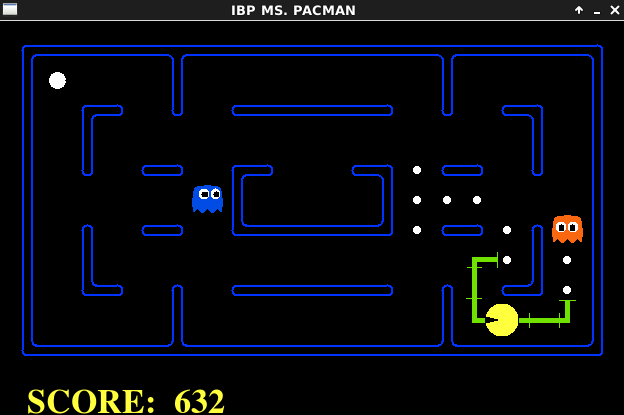
\includegraphics{img/reflexthrashV.png}}
  \caption{Na obrázku lze vidět problematické místo pro ohodnocovací funkci agenta. Zelená čára reprezentuje stejnou manhattonovskou vzdálenost (o velikosti 3 políčka) mezi Ms. Pacman a nebližší kuličkou jídla.}
  \label{img:reflexthrashV}
\end{center}
\end{figure}

\section{Základní algorimy}
Základní algoritmy vč. reflexivního agenta jsou implementovány pro problém Ms. Pacman (a její různé \textbf{mapy bludiště} ze složky \texttt{src/layouts}) a jejich spuštění je detailně popsáno v přílohové části manuál \ref{priloha:manualp}. Algoritmy musí mít přehled, která strana je na tahu na základě indexu agenta a také o kolikátou vrstvu střídání Ms. Pacman vs. (1-$N$) duchů se jedná -- to zajišťuje jejich instanční proměnná \texttt{depth}. Pro časovou a výpočetní únosnost byla zvolena výchozí hodnota hloubky \texttt{depth} 2. Pro správnou funkcionalitu frameworkového návrhu získávání agentem zvolené akce metodou \texttt{getAction} se musí průběžně vracet nejen aktuální hodnota uzlu, ale i \textbf{akce}, která je pro daného agenta optimální (zda se jedná o maximalizační nebo minimalizační vrstvu (popř. včetně vlivu pravděpodobnosti u \texttt{ExpectimaxAgent})). Během vyhodnocování se souběžně pracuje s polem \texttt{[akce,hodnota]} a následně, až se algoritmy dostanou ke kořeni (agent Ms. Pacman) je vrácena pouze vyhodnocená akce, jež má agent právě provést.
Během implementace se ukázalo, že je názornější zakázat agentovi se zastavit (vynechat z vyhodnocení přípustnou akci \texttt{STOP}), aby v případech s podobným ohodnocením stavů, jako u reflexivního agenta bylo jasně vidět zacyklené chování agenta.
Výňatek z kódu \ref{code:abaction} ukazuje metodu \texttt{getAction} pro získání akce u agenta \texttt{AlphaBetaAgent}\footnote{Komentáře v kódu jsou psány anglicky, aby navazovaly na framework. Výňatek má komentáře přeloženy.}.

\begin{python}[label={code:abaction}]
def getAction(self, gameState):
   # ziskani hodnot z metody AlfaBeta objektu AlphaBetaAgent
   value = self.AlphaBeta(gameState, self.index, 0,
   float("-inf"), float("inf")) # inicializace parametru alfa a beta
   return value[0] # vraceni akce pro hru
\end{python}

\subsection*{Ohodnocovací funkce}
Vyhodnocovací funkce následníků \texttt{evaluationFunction} pro agenty \texttt{MinimaxAgent} a \\* \texttt{AlphaBetaAgent} je založena na jejich skóre, jak již bylo zmíněno v sekci \ref{navrh:minabmaxy}. Tato funkce se měla původně nasadit i na agenta \texttt{ExpectimaxAgent}, avšak během implementace přišel nový nápad, a sice využití lepší vyhodnocovací funkce \texttt{betterEvaluationFunction} pro stav tohoto agenta. Tento nápad byl dodatečně doplněn i do návrhové části agenta v sekci \ref{navrh:expectimax}. Funkce implementuje lineární kombinaci hodnot dle faktorů ovlivňujících stav Ms. Pacman. Funkce je založena především na kombinaci proměnných:
\begin{itemize}
  \item \texttt{foodFactor} -- pozitivně vnímá: vzdálenost nejbližšího jídla, počet zbývajících power-upů, počet zbývajících kuliček jídla (nutnost odečítat nebo být dělitelem, aby platilo: Čím menší hodnota, tedy vzdálenost jídla atp., tím větší a potažmo lepší bude \texttt{foodFactor}) 
  \item \texttt{ghostFactor} -- pozitivně vnímá: vystrašený chytitelný duch; negativně vnímá: vzdálenost nejbližšího nevystrašeného ducha menší jak 4 políčka (přičtením duchovy vzdálenosti tak, aby platilo: Čím je blíž, tím je \texttt{ghostFactor} nižší) atp.
\end{itemize}
Dohromady tyto faktory společně se skórem stavu dávají finální ohodnocení stavu \texttt{value}, které prochází algoritmem Expectimax.

\section{Framework a MDP problematika}
Hlavním objektem pro pokročilé agenty je abstraktní objekt \texttt{ValueEstimationAgent} (dědící od základní třídy \texttt{Agent}; v souboru \texttt{learningAgents.py}). Tento agent slouží především pro propojení prostředí problému (Ms. Pacman, gridworld) s Q-hodnotami párů (stav,akce), dále propojení stavu s jeho V-hodnotou ($V(s)$) a nakonec propojení výsledných hodnot s výslednou nalezenou strategiií ($\pi(s)$).
Agenti od něj dále dědí a přetěžují základní metody:
\begin{itemize}
\item \texttt{getQValue(state,action)} -- vrací Q-hodnotu pro pár (stav,akce),
\item \texttt{getValue(state)} -- vrací V-hodnotu pro stav,
\item \texttt{getPolicy(state)} -- vrací strategii (akci) pro daný stav po i, při vyhodnocení chování agenta daným algoritmem na základě \texttt{getQValue(state,action)},
\item \texttt{getAction(state)} -- vrací strategii pro stav (přímo bez \textit{exploration}, používáno prostředím pro inicializaci).
\end{itemize}
\textbf{ValueIterationAgent} (ze souboru \texttt{valueIterationAgents.py}) navíc potřebuje pro svoje chování model (přechodová funkce T, odměnová funkce R) a využívá pro to abstrakní třídu \texttt{MarkovDecisionProcess} ze souboru \texttt{mdp.py}. \texttt{MarkovDecisionProcess} je dále využíváná prostředím (třída \texttt{Gridworld} reprezentující gridworld problémy v souboru \texttt{gridworld.py}), které napojuje své stavy (souřadnice polí mřížky a jejich odměna) a akce pomocí metody \texttt{getTransitionStatesAndProbs(state, action)} na jejich pravděpodobnost výskytu. Metoda vrací list párů $((s,a,s^\prime),T(s,a,s^\prime))$, tedy (následník aktuálního stavu,jeho přechodová funkce = pravděpodobnost výskytu).
Abstraktní \texttt{ReinforcementAgent}, který je základním objektem pro všechny agenty strojového učení, se stará o chování učícího se agenta během průběhu jednotlivých epizod tréninku a během provádění výsledné strategie, dále řeší základní vstupní parametry pro agenty jako nastavení počtu epizod k provedení (instanční proměnná \texttt{numTraining}) atp. a v případě Ms. Pacman spravuje průběžný a finální výpis během epizod. K výpisu pro Ms. Pacman je potřeba uchovávat akumulované odměny z tréninku \texttt{accumTrainRewards} a akumulované odměny z testování získané strategie tréninku \texttt{accumTestRewards}. Ty se nakonec podělí počtem provedených epizod (tréninku nebo testování) a takto vyjdou průměry odměn pro výpis\footnote{o výpis pro gridworld problémy se stará metoda \texttt{runEpisode} z \texttt{gridworld.py} během provádění epizod}.
Důležitými metodami jsou:
\begin{itemize}
\item \texttt{observeTransition(state,action,nextState,deltaReward)} -- voláno prostředím (Ms. Pacman, gridworld), které informuje agenta, že je získána nová hodnota přechodové funkce (nový přechod do stavu po akci), aby se následně vyvolala \textbf{aktualizace (update) Q-hodnot} a předala se mu okamžitá odměna jako rozdíl skóre následníka vůči aktuálnímu stavu (proměnná \texttt{deltaReward}),
\item \texttt{update(state, action, nextState, reward)} -- aktualizace nových odhadů Q-hodnot na základě získané okamžité odměny přechodu \texttt{delyaReward}; agenti tuto metodu přetěžují ve vlastním objektu,
\item \texttt{final(state)} -- finální výpis pro Ms. Pacman.
\end{itemize}
\texttt{ReinforcementAgent} staví na odhadu tabulky Q-Hodnot, protože neobsahuje model a je rodičem objektu řešící Q-Learning pro gridworld problémy \texttt{QLearningAgent}. Podobný agent, avšak s odlišnými vstupními parametry pro problém Ms. Pacman jsou \texttt{PacmanQAgent} a nakonec dále dědící \texttt{ApproximateQAgent}, který navíc implementuje algoritmus Aproximační Q-learning a využívá u toho třídy \texttt{FeatureExtractor} pro implementaci vektoru vlastností pro Ms. Pacman.

\section{Value Iteration agent a gridworld problémy}
Objekt \texttt{ValueIterationAgent} provádí své vyhodnocení V-Hodnot již v konstruktoru a to do pevného počtu iterací. Důvodem opuštění podmínky konvergence je především možnost pozorovat kolik iterací stačí pro optimalitu strategie. Z vypočetních (nutnost stanovit model) a názorných důvodů je tento agent zobrazen výhradně formou \textbf{gridworld} problémů (mřížky hodnot začínající se definovanými odměnami spustitelné pomocí \texttt{gridworld.py} -- viz manuál \ref{priloha:manualg}), kde jedno políčko po provedení metody ukazuje svou výslednou V-hodnotu (po provedení počtu daných iterací), po zmáčknutí klávesy (např. "Q") své 4 Q-hodnoty pro každý směr/akci a agent následně provede stanovený počet epizod svého chování (agentovo provedení vyhodnocené strategie). 
Průběh implementace tohoto agenta byla pravděpodobně nejdelší co vůbec do praktického pochopení iterativního charakteru V-hodnot. Během implementace se ukázalo, že vektor hodnot stavů stačí ukládat pouze do jedné proměné a po každé iteraci jej znovu přepisovat. Původní myšlenka totiž byla, že vektor si bude ukládat i jakousi částečnou historii stavů včetně Q-hodnot, ze kterých jsou V-hodnoty sestavovány. Tento nápad byl po naprogramování okamžitě zavržen vzhledem k jeho výpočetní náročnosti a celkové nerelevantnosti k MDP problémům. Vždyť právě myšlenka MDP je pouze vycházet z přechodů z aktuálních stavů do jejich následníků. Ustanovila se tedy jedna nejdůležitější instanční proměnná \texttt{values} sloužící pro uložení aktuálních V-hodnot ve formě \textit{slovníku} pro každé pole mřížky a její aktuální V-hodnotu např. [(0,1):-10.0,(5,3):0.0]). Po každé iteraci se V-Hodnoty \textbf{přepíší} na aktuální, to lze vidět na výňatku z kódu konstruktoru agenta \ref{code:valagent}:

\begin{python}[label={code:valagent}]
# inicializace instancnich promennych
self.mdp = mdp			# MDP model pro gridworld
self.discount = discount     # gamma
self.iterations = iterations # pocet iteraci
self.values = util.Counter() # slovnik V-hodnot

for k in range(iterations):
   futureValues = self.values.copy()   # $V_{k+1} \leftarrow V_k$
   for state in self.mdp.getStates():  # pro kazdy stav modelu (1 pole mrizky)
      # ziskej pripustne akce pro stav
      actions = self.mdp.getPossibleActions(state)
      # pokud je stav terminalni, uloz $V[stav]_{k+1} = 0$ a pokracuj na novy stav
      if mdp.isTerminal(state) or len(actions) == 0:
         futureValues[state] = 0
         continue
      # ziskej nejlepsi hodnotu z odhadu uzitku vsech akci prechodu
      # = z Q-hodnot
      value = float("-inf")
      for action in actions:
         # suma Q-hodnot pro kazdou akci
         expectedQValue = 0.0
         # napojení na model -- ziskani Q-hodnot pro stav
         expectedQValue = self.getQValue(state, action)
         if expectedQValue > value:
            value = expectedQValue
      # $V^*(s)$ -- nejlepsi hodnota ocekavaneho budouciho uzitku
      futureValues[state] = value
   self.values = futureValues # prepis V-Hodnoty na aktualni
\end{python}

Výsledné provedení chování agenta je podobné jako u Q-Learning Agentů -- viz výňatek z kódu \ref{code:qpolicy}, avšak lze pro optimalitu strategie provést až po provedení iterací \texttt{values} v konstruktoru agenta \ref{code:valagent}. Agent neprovádí trénink (nevyužívá $\epsilon-greedy$), takže se vždy provede nejlepší možná akce stavu na základě odhadů Q-hodnot z modelu (které jsou sestaveny dle pseudokódu \ref{alg:valiterq}) pomocí volání metody na získání strategie \texttt{getPolicy(state)}.

Framework nabízí hned několik \textbf{gridworld problémů}, avšak nejzajímavějšími jsou:
\begin{itemize}
  \item \texttt{BookGrid}, který byl již ukázán v teoretické části (obrázky \ref{img:policy} a \ref{img:qvals}).
  \item \texttt{DiscountGrid}, problém zahrnující 2 terminální cíle (s pozitivní odměnou) a útes 4 terminálních stavů s velmi negativní odměnou. Agent se potýká s tím, zda jít delší bezpečnou cestou, nebo kratší riskantnější cestou podél útesu a také s faktem, že cíle mají rozdílné odměny (vzdálenější má hodnotnější odměnu). Rozdílné chování agenta je ovlivňováno instanční proměnnou \texttt{gamma} (koeficient odměny), počtem provedených iterací a stochastičností agentových akcí. Proto je tento problém ideální na zkoumání.
  \item \texttt{BridgeGrid}, problém modelující most mezi pozitivními terminálními cíli podél útesů z každé strany. Ukázku tohoto gridworld problému lze vidět na obrázku \ref{img:bridgeGridDefault}.
\end{itemize}
Tyto problémy budou experimenálně otestovány i Q-Learning agentem \texttt{QLearningAgent} v následující kapitole \ref{exper}.

\begin{figure}[!htbp]
\begin{center}
  \scalebox{0.35}{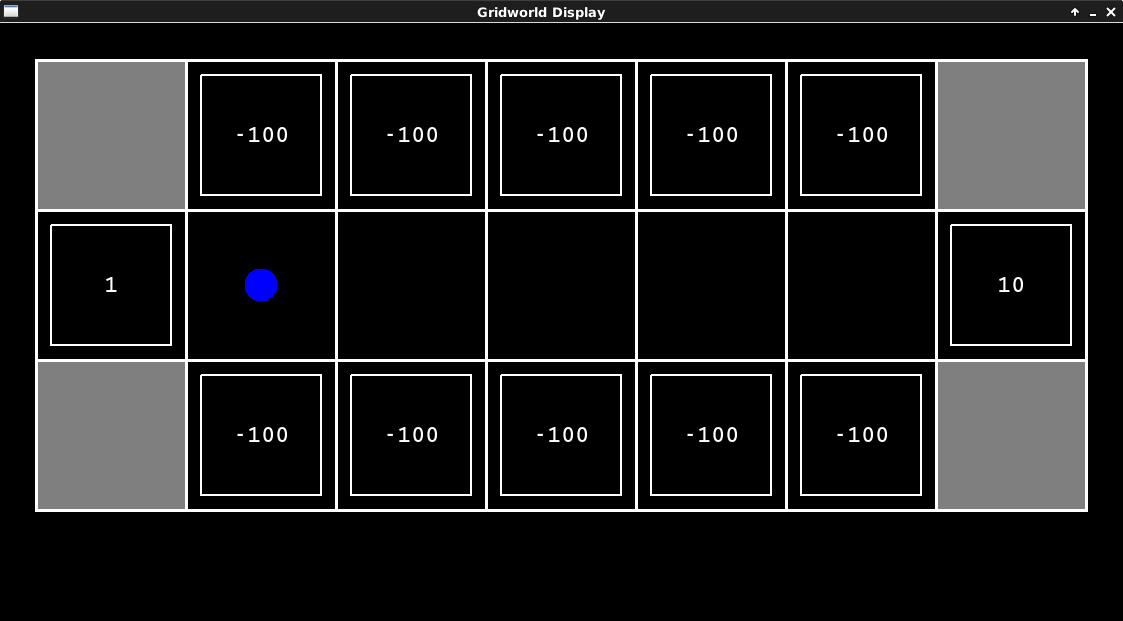
\includegraphics{img/bridgeGridDefault.png}}
  \caption{Screenshot počátečního modelu gridworld problému \texttt{BridgeGrid} pro Value Iteration agenta (Q-Learning agent toto ohodnocení odměn stavů nemá) ukazuje stavy a jejich odměnu. Agent je reprezentovaný modrou tečkou.}
  \label{img:bridgeGridDefault}
\end{center}
\end{figure}

\section{Q-Learning agenti}
Jelikož bude Q-Learning nasazen jak na gridworld problémy, tak na Ms. Pacman, je potřeba tyto agenty rozlišovat na základě jejich vstupních parametrů, které byly poskytnuty frameworkem:
\begin{itemize}
\item pro \texttt{QLearningAgent}: alpha = 0.5, epsilon = 0.5, gamma = 1.
\item pro \texttt{PacmanQAgent} a \texttt{ApproximateQAgent}: alpha = 0.2, epsilon = 0.05, gamma = 0.8.
\end{itemize}
Po analýze těchto parametrů se došlo k těmto závěrům:
\begin{enumerate}
\item Parametry pro gridworld problémy jsou nastaveny do výchozích hodnot, které budou během experimentování často měněny, takže příliš nezáleží jejich výchozí hodnotách.
\item Parametry pro Ms. Pacman byly experimentálně zjištěny autory frameworku tak, aby se Ms. Pacman učila spíše pomaleji (velmi malá hodnota parametru alpha) a měla následně uživatelem nastavený delší trénink, spíše málo experimentovala (vliv malé hodnoty parametru epsilon) a snažila se spíše co nejrychleji sníst kuličky jídla (vliv sníženého parametru gamma).
\end{enumerate}
Jak již bylo řešeno v \ref{navrh:qlearnagent}, tito agenti si musí model odhadnout sami na základě získaných odměn při výběru akcí na pomocí \textit{exporation/exploitation ratio}. Tento poměr je dán instanční proměnnou \texttt{epsilon} a předán funkci \texttt{flipCoin}, jež určí finální rozhodnutí výběru akce. Pokud se má provést aktuální akce, volá se pro stav metoda \texttt{getPolicy(state)}, která na základě tabulky Q-hodnot (Q-hodnota je vracena přímo opět metodou \texttt{getQValue(state, action)} narozdíl od \textbf{ValueIterationAgent}, který si Q-hodnotu musí nejdříve sestavit na základě modelu, jak je vidět v návrhu pseudokódu \ref{alg:valiterq}).

Pro názornost si lze uvést výňatek z kódu (část vyhodnocení strategie pro stav během tréninku Q-Learning agentů) \ref{code:qpolicy}. Agenti si ukládají pouze tabulku aktuálních odhadů Q-hodnot jako slovník \texttt{qValues} pro každý pár \texttt{(state,action)} a vychází z návrhu pseudokódu~\ref{alg:qlearn}.
\newline POZNÁMKA: V jazyce Python je instance třídy metodě posílána automaticky, avšak přijímána již automaticky není. Proto je potřeba napsat do argumentů funkce klíčové slovo \textit{self}.

\begin{python}[label={code:qpolicy}]
def getAction(self, state):
   actions = self.getLegalActions(state)
   # terminalni stav
   if len(actions) == 0:
      return None
   # pravdepodobnost dana $\epsilon-greedy$ 
   if flipCoin(self.epsilon):
      # prozkoumavani novych stavu behem treninku
      return random.choice(actions) # nahoda akci pro stav (\textit{exploration})
   else:
      # nejlepsi mozna akce na zaklade tabulky odhadu Q-hodnot (\textit{exploitation})
      return self.getPolicy(state)
\end{python}

Již během implementace bylo zjištěno, že vzhledem k množství párů (stav,akce) bude Q-Learning agent Ms. Pacman (\texttt{PacmanQAgent}) testován spíše na menších mapách a určitě bude potřeba nastavit větší počet epizod tréninku, pro ukázku lze uvést příklad: \ref{img:smallL}.
\begin{figure}[!htbp]
\begin{center}
  \scalebox{0.6}{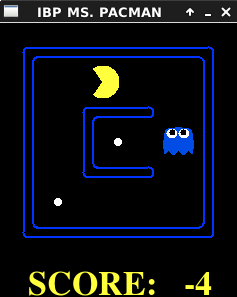
\includegraphics{img/smallL.png}}
  \caption{Screenshot menší mapy (\texttt{smallGrid}) pro Ms. Pacman.}
  \label{img:smallL}
\end{center}
\end{figure}

\section{Aproximační Q-Learning agent}
\label{impl:aproxq}
Agent \texttt{ApproximateQAgent} využívá proměnnou \texttt{weights}, tedy slovník párů \textit{(vlastnost,váha)} (výchozí hodnota váh je rovna $0.0$), kterými se pronásobí její hodnota. Hodnota vlastnosti je získána voláním metody \texttt{getFeatures(state, action)} objektu \texttt{BetterExtractor} (dědící ze základního objektu \texttt{FeatureExtractor})), který ji vrací opět formou slovníku párů \textit{(vlastnost,hodnota)}, které jsou uloženy v instanční proměnné objektu \texttt{features}. Metoda \texttt{getPolicy(state)} zůstává stejná (získání nejlepší možné akce pro stav), avšak místo aby metoda stavěla na získání uložené Q-hodnoty z tabulky (pomocí metody \\* \texttt{getQValue(state, action)}), Q-hodnota se sestaví pomocí váh vektoru vlastností, jak je vidět na výňatku z kódu stejnojmenné metody ~\ref{code:aqqval}.
\begin{python}[label={code:aqqval}]
def getQValue(state, action):
   qvalue = 0.0
   # ziskani vektoru vlastnosti s jejich hodnotami
   features = self.featExtractor.getFeatures(state, action)
   for i in features: # iteruj po vlastnosti
      # pronasob váhu vlastnosti s jeji hodnotou
      qvalue += self.getWeights()[i] * features[i]
   return qvalue
\end{python}
Aktualizace váh vlastností na základě nového přechodu (opět voláno rodičovskou funkcí \\* \texttt{observeTransition(state, action, nextState, deltaReward)}) pak vypadá takto:
\begin{python}
def update(self, state, action, nextState, reward):

   # rozdíl vzorků $= \left [ r + \gamma \max_{a^\prime}Q(s^\prime,a^\prime) \right] - Q(s,a)  $
   difference = (reward + self.discount * self.getValue(nextState)) 
                - self.getQValue(state, action)
   # ziskani vektoru vlastnosti s jejich hodnotami
   features = self.featExtractor.getFeatures(state, action)
   for i in features:
      # samotna aktualizace váhy dané vlastnosti
      self.getWeights()[i] += self.alpha * difference * features[i]
\end{python}

Pravděpodobně nejdůležitější pro celého agenta je kvalitní stanovení hodnot pro stav ve vektoru vlastností. Framework nabízí několik typů extraktorů vlastností pro vektor vlastností -- např. \texttt{CoordinateExtractor}, který je založený na triviálních vlastnostech typu stav, akce, koordináty stavu na gridworldu Ms. Pacman. Jelikož jsou extraktory navázány na MDP, je k dispozici informace o aktuálním stavu a jeho následníkovi po dané akci. Lze tedy generalizovat daný stav ve hře pomocí nahlédnutí na stav hry jeho následníka raději než staticky popisovat koordináty atp. Během návrhu vektoru vlastností \ref{navrh:approxqlearnagent} se počítalo až se sedmi vlastnosmi, které popíšou stav následníka. Během implementace se však ukázalo, že aproximace takovým množstvím vlastností není efektivní a některé vlastnosti, např. vzdálenost power-upu nejsou ze stavu následníka vůbec dosažitelné. U počítání vzdálenosti power-upu je potřeba větší rozhled, než pouze následníkova hloubka o velikosti 1, tudíž by byla potřeba metoda prohledávání stavového prostoru. Nalezení hodnoty této vlastnosti by pak bylo příliš vypočetně náročné vzhledem k tomu, že pravděpodobnost její změny je nižší a vlastnost nemá takový vliv na výsledný vektor. Mnohem účinnější je vzít základní dostupné vlastnosti  a logicky je spolu prokombinovat. Vlastnosti používáné objektem \texttt{BetterExtractor} se tedy mezi sebou navíc logicky ovlivňují a relevantněji popisují aktuální dění stavu hry. Tento extraktor vylepšuje frameworkový \texttt{SimpleExtractor} především tím, že bere v potaz i stav duchů. Vektor vlastností objektu \texttt{SimpleExtractor} se primárně zaměřuje na všechny duchy bez rozdílu. Agent pak ale bohužel naráží na zbytečné vyhýbání se vystrašeným duchům, jež by mohl sníst. \texttt{BetterExtractor} tedy navíc bere v potaz i vystrašenost duchů a blízkost power-upů. Vektor vlastností objektu \texttt{BetterExtractor} popisuje vlastnosti\footnote{hodnota vlastností se také musela pomenšit dělením tak, aby se předešlo divergenci hodnot.}:
\begin{itemize}
\item \texttt{"active-ghosts-1-step-away"} - počet aktivních duchů z okolí následníka (vzdálenost 1 krok),
\item \texttt{"scared-ghosts-1-step-away"} - počet vystrašených duchů z okolí následníka,
\item \texttt{"can-eat"} - Ms. Pacman může jíst jídlo a nemusí se bát aktivních duchů,
\item \texttt{"powerup"} - v okolí následníka je powerup a je blízko vystrašený duch,
\item \texttt{"closest-food"} - vzdálenost nejbližšího jídla.
\end{itemize}
Samotná ukázka logické návaznosti vlastností je vidět na výňatku z kódu~\ref{code:aqlbetterfeature}. Výňatek demonstruje, jak jednoduše lze generalizovat stav tak složitého problému jako je Ms. Pacman, aniž by bylo potřeba konkrétně popsat všechny informace o stavu hry. Pouze stačí 5 vlastností s hodnotami a jejich váhy. Není potřeba tabulky Q-hodnot pro každý pár (stav,akce), ani není potřeba iteračně přepočítávat V-hodnoty každého stavu na základě Q-hodnot akcí. Aproximační Q-Learning jde nasadit i na větší mapy a v experimentální části se i ukáže o kolik méně je potřeba tréninku k aproximaci stavů oproti sestavení celé tabulky Q-hodnot. \newline POZNÁMKA: proměnná \texttt{numGhosts} označuje počet duchů, \texttt{(next\_x, next\_y)} jsou koordináty následníka na gridworldu Ms.~Pacman, metoda \texttt{getLegalNeighbors(gPos, walls)} vrací list koordinát dostupných polí z okolí předané pozice \texttt{gPos}.
\begin{python}[label={code:aqlbetterfeature}]
for i in range(0,numGhosts):
   gPos = state.getGhostPosition(i+1%(numGhosts+1)) # ziskani pozice ducha
   g = state.getGhostState(i+1%(numGhosts+1)) 	# ziskani duchova stavu
   # zjisti zda je duchova pozice v okoli následnika
   if (next_x, next_y) in Actions.getLegalNeighbors(gPos, walls):
      if g.scaredTimer < 1:   # duch aktivni
         features["active-ghosts-1-step-away"] += 1
      else:                   # duch je vystraseny
         features["scared-ghosts-1-step-away"] += 1

# pokud neni aktivni duch blízko a naslednik obsahuje jidlo
if not features["active-ghosts-1-step-away"] and food[next_x][next_y]:
   features["can-eat"] = 1.0

# pokud naslednik obsahuje powerup a je blizko aktivni duch, jez bude po sebrani
# power-upu ke snezeni
if((next_x, next_y) in powerups and not 
features["active-ghosts-1-step-away"]):
    features["powerup"] = 1.0
\end{python}

\chapter{Experimenty a srovnání agentů}
\label{exper}
Agenty lze srovnat nejlépe podle dosaženého herního skóre.
\section{Srovnání z hlediska skóre}
\section{Srovnání z hlediska času}
\section{Srovnání z hlediska vypočetní náročnosti}
\section{Výsledky}
učící křivka (x:skóre,y:počet tréninku)

\chapter{Závěr}
-PŘEPSAT-
Cílem toho semestrálního projektu bylo nastudovat problematiku metod hraní her ve vztahu k učícímu agentovi pro hru Ms. Pacman a navrhnout metodu řešení problému. Ms. Pacman. Nastudování teorie pomohlo především k definici a klasifikaci samotné hry jako problému umělé inteligence, a následném stanovení návrhu řešení problematiky metodou Aproximační Q-Learning. Tato metoda řeší stochastické chování duchů a pomůže výrazně eliminovat problém velké vypočetní náročnosti stavového prostoru Ms. Pacman. Jak si metoda s takto složitou problematikou poradí bude nejlépe vidět při srovnání její efektivity například s metodou Expectimax. Práce mě naučila především nebát se složitějších matematických vzorců a problémů a též určitý vhled do možností strojového učení.

It have been shown that value iteration algorithm performs faster and better
as compared to both the variants of Q-learning algorithm. However in more
realistic settings, the value iteration might not be able to find the optimal
solution while the Q-learning algorithm would perform better. It is also
shown that the implementation of Q-learning algorithm that uses function
approximator, though slow, would be better in long run as compared to the
version that uses lookup table. This would happen because as the state space
grows, the memory requirement for storing various states would also grow
exponentially rendering the lookup table version useless.
The limitation of our approach was that we used linea

